\chapter{ RESULTS AND DISCUSSION}

%\section{Introduction}

This section presents the results and discussion of the proposed control framework, beginning with model verification to establish the accuracy and reliability of the developed quadrotor dynamics. The verified model provides a sound basis for controller design and performance evaluation. Subsequently, the effectiveness of the Particle Swarm Optimization (PSO) approach in tuning controller parameters is demonstrated, highlighting improvements in convergence and robustness. Finally, trajectory tracking results are analyzed to assess the controller’s ability to achieve precise and stable motion under varying conditions. Together, these results provide a comprehensive validation of the proposed method and its practical applicability.

\section{Verification of Quadrotor Dynamic Model}

%This step in the process of designing control system is also known as Quantitative analyses of the derived model of the system. To verify feasibility of the derived mathematical model of Quadrotor dynamics, simulations were conducted under MATLAB\textsuperscript{\textregistered} Simulink software by using parameter values presented in Table~\ref{tab:quad_params}

%This stage of control system design is referred to as \textit{quantitative analysis} of the derived model. 
To verify the feasibility of the quadrotor dynamic model, simulations were performed in 
MATLAB\textsuperscript{\textregistered} Simulink using the parameter values listed in Table~\ref{tab:quad_params}.


\begin{table}[h!]
\centering
\caption{Specifications for the Quadrotor model design ~\cite{ahmed2018sliding},\cite{bernard2017dynamic}}
\label{tab:quad_params}
\begin{tabular}{|c|l|c|c|}
\hline
\textbf{Symbol} & \textbf{Description} & \textbf{Unit} & \textbf{Value} \\ \hline
$g$     & Acceleration due to gravity              & $ms^{-2}$  & 9.81 \\ \hline
$m$     & Mass of Quadrotor                        & $Kg$       & 0.468 \\ \hline
$J_{xx}$ & Body moment of inertia around the X-axis & $Nms^2$    & $4.856 \times 10^{-3}$ \\ \hline
$J_{yy}$ & Body moment of inertia around the Y-axis & $Nms^2$    & $4.856 \times 10^{-3}$ \\ \hline
$J_{zz}$ & Body moment of inertia around the Z-axis & $Nms^2$    & $8.801 \times 10^{-3}$ \\ \hline
$\ell$   & Length of Quadrotor arm                 & m          & 0.225 \\ \hline
$b$     & Thrust coefficient                       & N/m/s      & $2.98 \times 10^{-6}$ \\ \hline
$d$     & Drag factor                              & $Nms^2$    & $1.140 \times 10^{-7}$ \\ \hline
$J_p$   & Rotor or propeller inertia               & $Nms^2$    & $3.357 \times 10^{-5}$ \\ \hline
$C_{\alpha} = C_{aq} = C_{ar}$ & Rotational drag coefficients & N/m/s & 0.25 \\ \hline
$C_{\alpha} = C_{av} = C_{az}$ & Translational drag coefficients & N/m/s & 0.2 \\ \hline
$R$     & Rotor or propeller Radius                & m          & 0.25 \\ \hline
$\gamma$& Correction factor                        & unit       & 0.083 \\ \hline
\end{tabular}
\end{table}

The open-loop system is analyzed by applying arbitrary inputs based on the following 
flight scenarios:

\begin{itemize}
  \item \textbf{Ascending or descending flight} is controlled by the total thrust $U_1$. 
  If $U_1 > mg$, the quadrotor ascends; if $U_1 < mg$, it descends; and if $U_1 = mg$, 
  it hovers at a constant altitude. In this case, all rotors spin at the same speed, 
  preventing rotational motion.

  \item \textbf{Lateral maneuvering} is achieved through roll and pitch torques 
  $U_2$ and $U_3$. According to Figure~\ref{fig:Quadrotor free body diagram}, if $U_2>0$, 
  the quadrotor rolls along the positive $y$-axis by increasing the speeds of rotors 1 
  and 4 while decreasing those of rotors 2 and 3. Similarly, if $U_3>0$, pitch motion 
  occurs along the negative $x$-axis by increasing the speeds of rotors 1 and 2 and 
  reducing those of rotors 3 and 4.

  \item \textbf{Heading control} is obtained by the yaw torque $U_4$. If $U_4>0$, the 
  quadrotor rotates clockwise about its center of gravity, increasing the speeds of 
  rotors 2 and 4 while decreasing those of rotors 1 and 3 to maintain altitude.
\end{itemize}

In this subsection, the quadrotor model is verified by applying open-loop control inputs. 
First, the vehicle ascends and then hovers at a specified altitude. From this hovering 
condition, roll, pitch, and yaw inputs are applied and MATLAB\textsuperscript{\textregistered} 
Simulink simulations are performed using the parameters listed in Table~\ref{tab:quad_params}.

\begin{itemize}
  \item The weight of the quadrotor is 
  $W = mg = 0.468 \times 9.81 = 4.591\,N$.
\end{itemize}

%\textbf{Ascending maneuver:} In the first scenario, the total thrust is set to 
%$U_1 = 4.7\,N$, which is greater than the gravitational force. As a result, the quadrotor ascends. All propellers rotate at the same speed, producing equal thrust, and therefore no rotational motion or lateral maneuvering along the $x$ or $y$ directions occurs, as illustrated in Figure~\ref{fig:Quad position and ground effect-ascending}.

\textbf{Ascending maneuver:} In the first scenario, the total thrust is set to 
$U_1 = 4.7\,N$ 

The ascending maneuver as shown in Figure~\ref{fig:Quad position and ground effect-ascending} provides a reliable benchmark for validating the proposed quadrotor model. When the applied thrust exceeds gravitational force, a smooth vertical rise is observed, with negligible lateral displacement, confirming stable position behavior along the \(z\)-axis. Both models capture this trend; however, the baseline model predicts a faster altitude increase, while the proposed model shows a more gradual ascent due to aerodynamic drag effects. The propeller speeds remain equal and converge to steady values, indicating balanced thrust generation across all rotors. Furthermore, the Euler angles (roll, pitch, and yaw) remain close to zero throughout the maneuver, confirming the absence of rotational motion and validating symmetry in the system. Angular velocities are also negligible, reinforcing stable attitude dynamics.  The enhanced model demonstrates improved physical realism and provides a more accurate representation of quadrotor behavior under practical flight conditions.



% NOTE INSERT FIGURE HERE
%\begin{figure}[h!]
    %\centering
   % 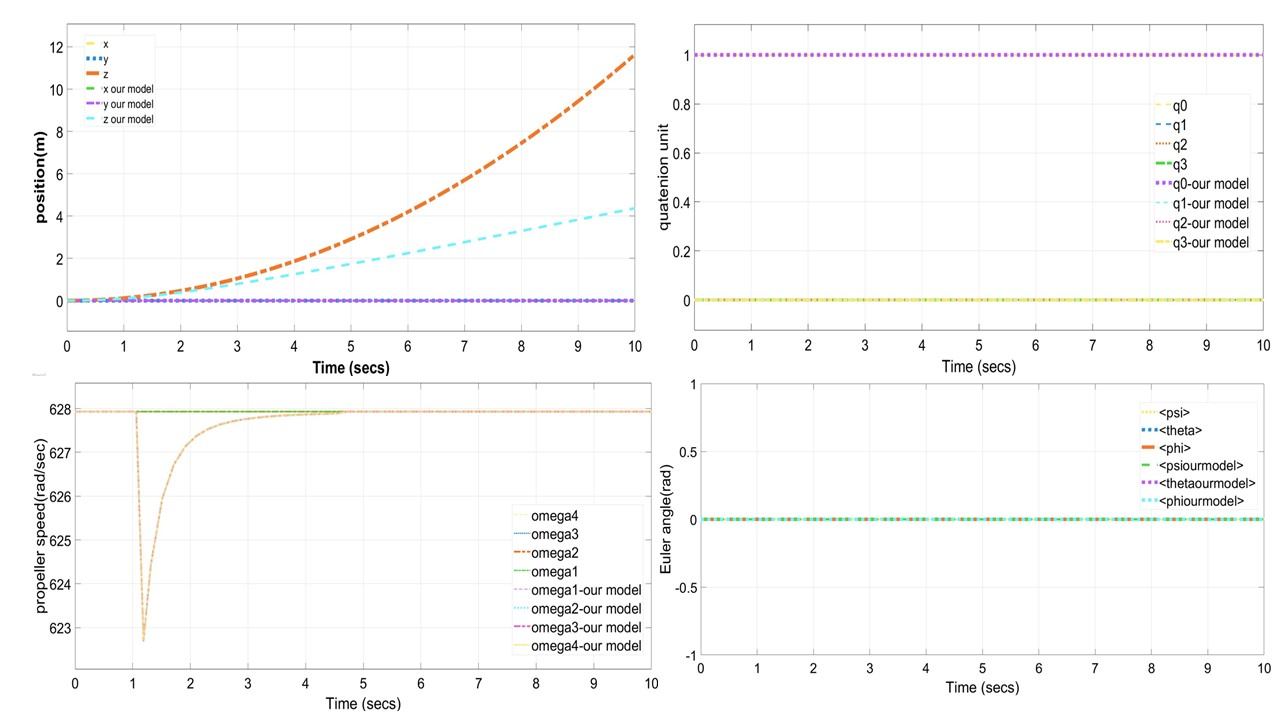
\includegraphics[width=1.0\linewidth]{figures/AscendingBest.jpg}
   % 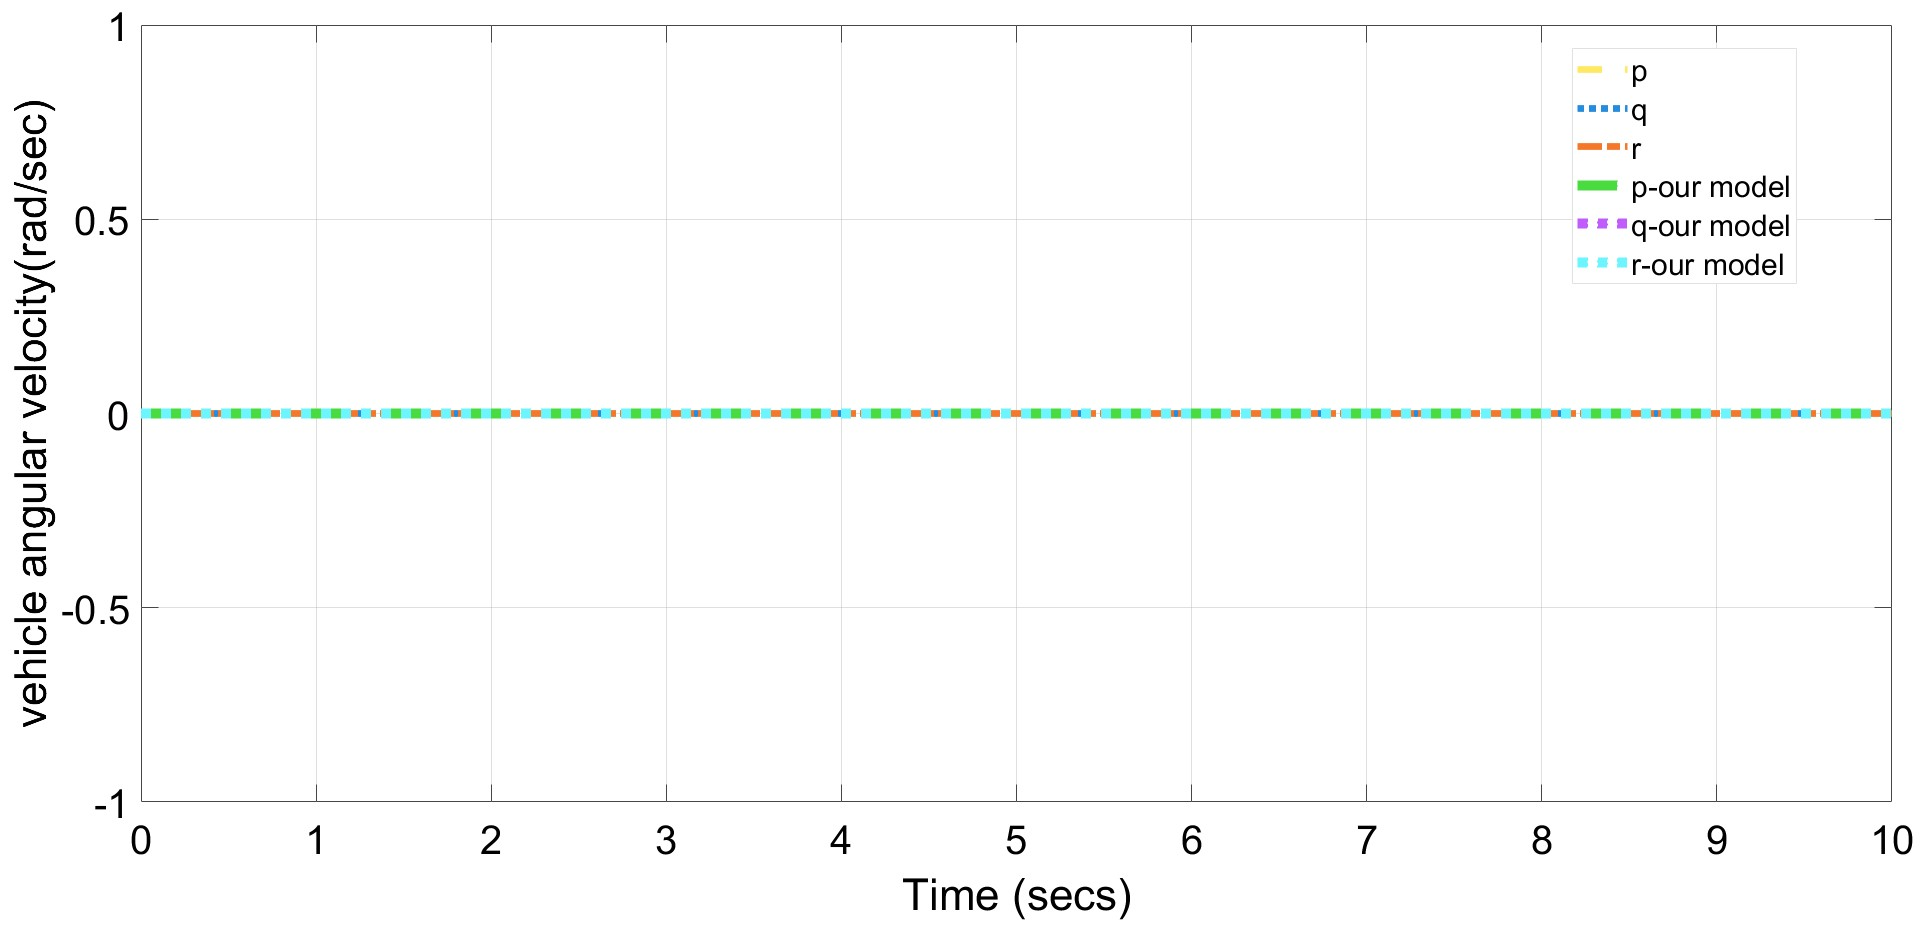
\includegraphics[width=1.0\linewidth]{figures/angularvelocityvehicle.jpg}
    %\caption{Quadrotor state for ascending maneuvering when $U_{1} > mg$}
   % \label{fig:Quad position and ground effect-ascending}
%\end{figure}

%%%%%%%%%%%%%%%%%%%%%%%%%%%%%%%%%%%%%%%%%%%
\begin{figure}[h!]
    \centering
    \begin{minipage}{0.48\linewidth}
        \centering
        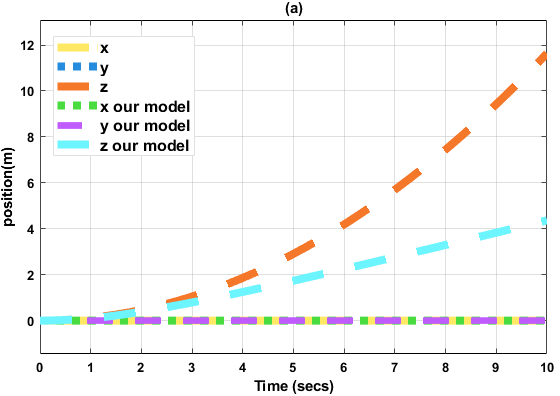
\includegraphics[width=1.0\linewidth]{figures/ascendingposition-BEST.png}
    \end{minipage}
    \hfill
    \begin{minipage}{0.48\linewidth}
        \centering
       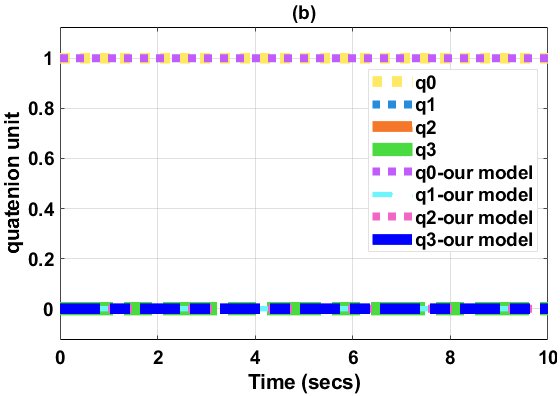
\includegraphics[width=1\linewidth]{figures/quaternion ascending-BEST.png}
    %\caption{Altitude controller diagram for maintaining desired quadrotor altitude}
    %\label{fig:attitude controller}
    \end{minipage}
\begin{minipage}{0.48\linewidth}
        \centering
        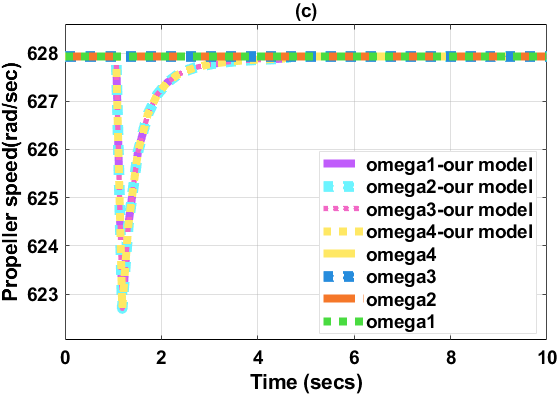
\includegraphics[width=1.0\linewidth]{figures/propeller speed-BEST.png}
    \end{minipage}
    \begin{minipage}{0.48\linewidth}
        \centering
        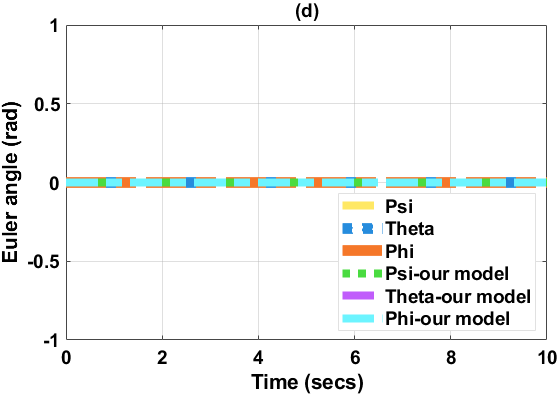
\includegraphics[width=1.0\linewidth]{figures/euler angle -BEST.png}
    \end{minipage}
    \begin{minipage}{0.48\linewidth}
        \centering
        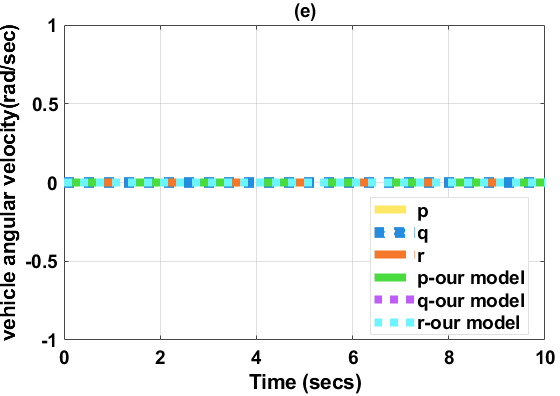
\includegraphics[width=1.0\linewidth]{figures/vehicle angular velocity-BEST.png}
    \end{minipage}
    \caption{Quadrotor state for ascending maneuvering when $U_{1} > mg$}
    \label{fig:Quad position and ground effect-ascending}
\end{figure}




%\textbf{Hovering state}: The quadrotor is first initialized at an altitude of $9\,\text{m}$. 
%Then the total thrust is set to $U_{1}=4.591\,N$, which is equal to the gravitational force. Under this condition, the quadrotor maintains a hovering state. Since no rotational motion occurs about any axis, the scalar part of the quaternion remains one while the vector components are zero, as illustrated in Figure~\ref{fig:hovering_state}.

\textbf{Hovering state}: The quadrotor is first initialized at an altitude of $9\,\text{m}$, 
then the total thrust is set to $U_{1}=4.591\,N$, which is equal to 
the gravitational force.
Figure ~\ref{fig:hovering_state} illustrates the hovering condition where thrust exactly balances the vehicle weight, resulting in a constant altitude. The position responses confirm this equilibrium, with the \(z\)-axis remaining steady at 9 m and no observable drift in the \(x\) and \(y\) directions for both models. Propeller speeds converge to identical constant values, indicating uniform thrust distribution required to sustain hover. The Euler angles remain at zero throughout, confirming the absence of roll, pitch, and yaw motion, while the quaternion representation maintains \(q_0 \approx 1\) and \(q_1, q_2, q_3 \approx 0\), consistent with a level orientation. Additionally, vehicle angular velocities are effectively zero, reflecting stable attitude dynamics. Both models exhibit similar steady-state behavior; however, the proposed model shows slightly smoother convergence, suggesting improved physical realism and damping due to aerodynamic effects, thereby enhancing confidence in its practical applicability.

%\begin{figure}[h!]
   % \centering
   % 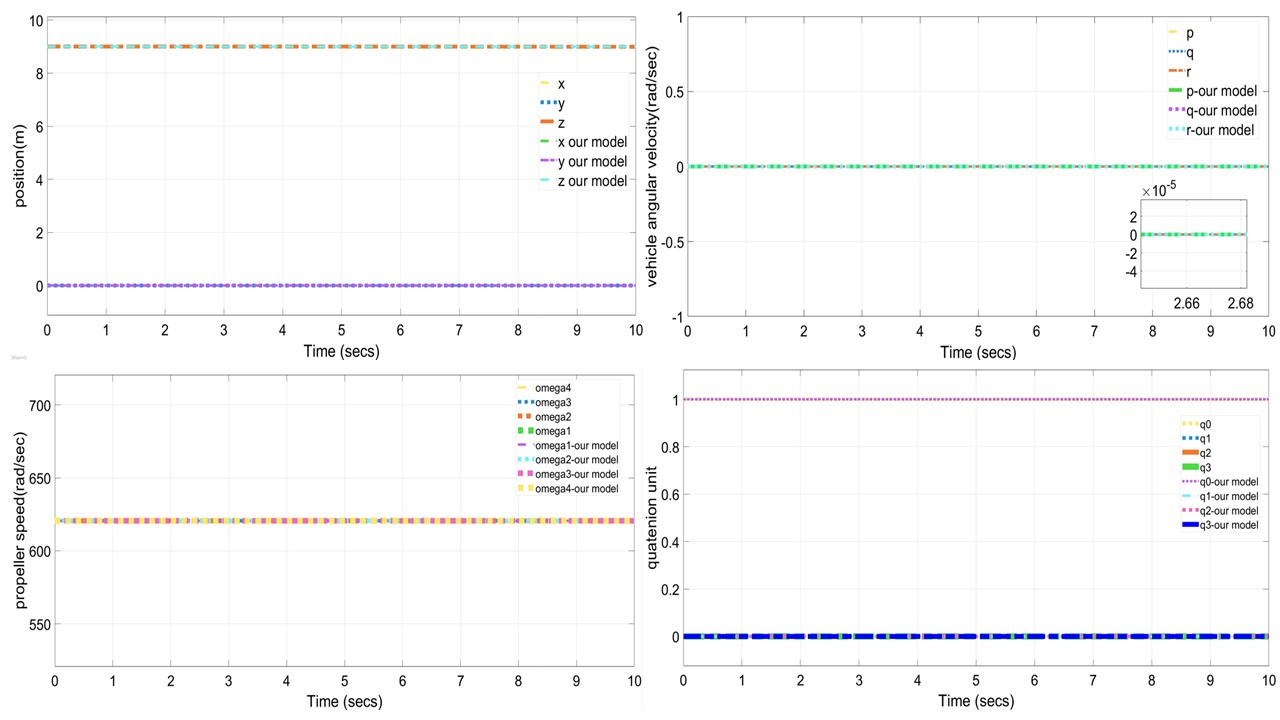
\includegraphics[width=1.0\linewidth]{figures/hoverfiguresvalidation.jpg}
    %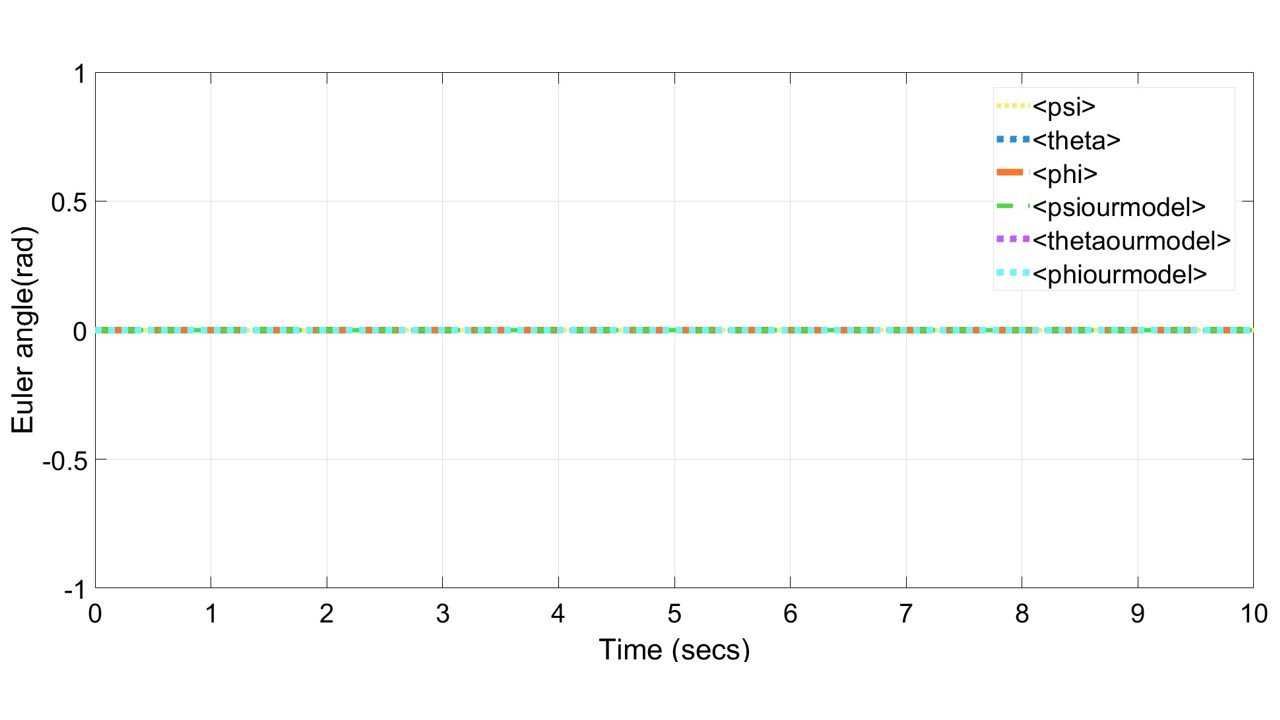
\includegraphics[width=1.0\linewidth]{figures/hovereulerangle.jpg}
   % \caption{At Hovering state when $U_{1} = mg$}
   % \label{fig:hovering_state}
%\end{figure}

\begin{figure}[h!]
    \centering
    \begin{minipage}{0.48\linewidth}
        \centering
        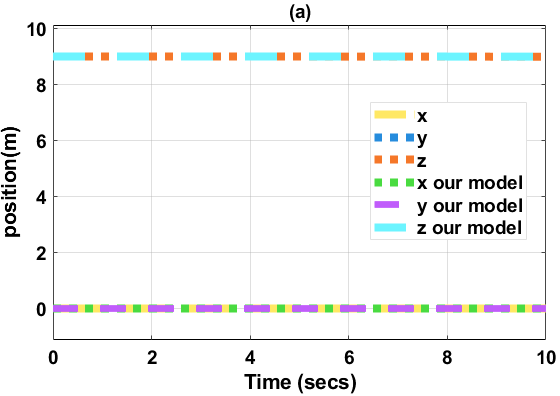
\includegraphics[width=1.0\linewidth]{figures/hover-position-BEST.png}
    \end{minipage}
    \hfill
    \begin{minipage}{0.48\linewidth}
        \centering
       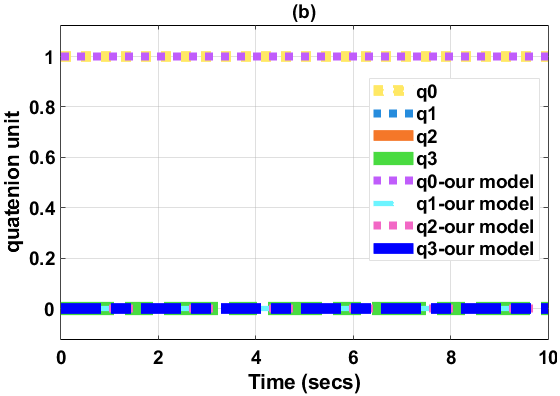
\includegraphics[width=1\linewidth]{figures/hover-quaternion-BEST.png}
    %\caption{Altitude controller diagram for maintaining desired quadrotor altitude}
    %\label{fig:attitude controller}
    \end{minipage}
\begin{minipage}{0.48\linewidth}
        \centering
        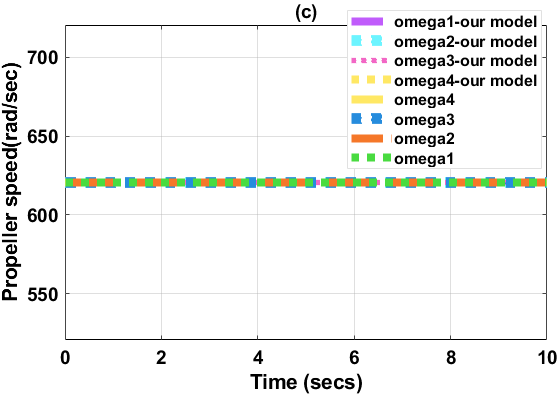
\includegraphics[width=1.0\linewidth]{figures/hover-propeller speed-BEST.png}
    \end{minipage}
    \begin{minipage}{0.48\linewidth}
        \centering
        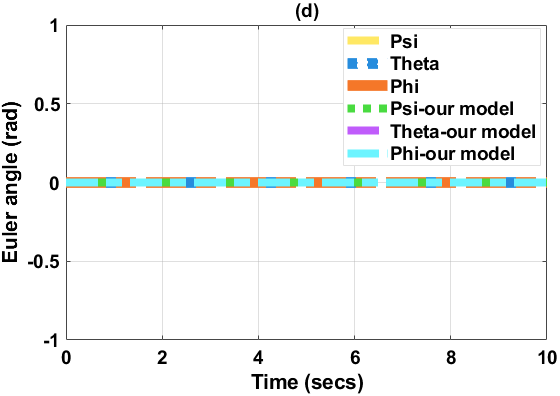
\includegraphics[width=1.0\linewidth]{figures/hover-euler-BEST.png}
    \end{minipage}
    \begin{minipage}{0.48\linewidth}
        \centering
        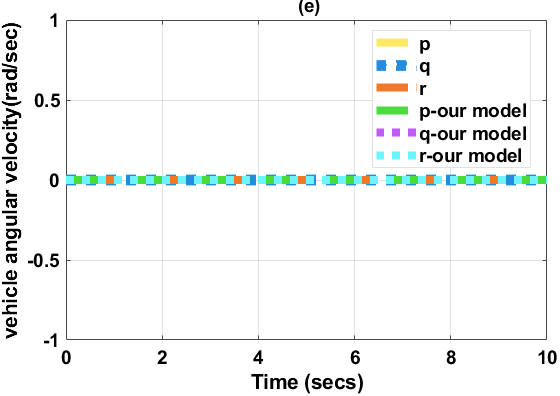
\includegraphics[width=1.0\linewidth]{figures/hover-vehicle velocity-BEST.png}
    \end{minipage}
    \caption{At Hovering state when $U_{1} = mg$}
   \label{fig:hovering_state}
\end{figure}



%\textbf{Roll rotation} :At the hovering state, the roll control torque is set to $U_{2}=0.2\,Nm$ while 
%keeping $U_{1}$ constant. This increases the speeds of motors 1 and 4 and 
%decreases those of motors 2 and 3, producing roll motion toward the positive 
%$y$-direction. Since the open-loop system is unstable, the quadrotor continues 
%to rotate about the $x$-axis. When the roll angle $\phi \geq \tfrac{\pi}{2}$, 
%the vehicle loses lift and falls rapidly to the ground, as illustrated in 
%Figure~\ref{fig:roll_rotation}.

\textbf{Roll rotation} :At the hovering state, the roll control torque is set to $U_{2}=0.2\,Nm$ while 
keeping $U_{1}$ constant, Figure ~\ref {fig:roll_rotation} confirms the expected open-loop roll instability of the quadrotor when a constant roll torque is applied during hover. The position responses show rapid altitude loss and growing lateral displacement, indicating that once the vehicle tilts significantly, part of the thrust is redirected from vertical support to rotational and lateral motion. This effect is more pronounced in the baseline model, whereas the proposed model exhibits a slightly moderated response due to the inclusion of aerodynamic and drag effects. The propeller speeds split into two groups, consistent with the roll command generation mechanism. The Euler angles reveal continuous growth of roll, while pitch and yaw remain comparatively small. The quaternion trajectories depart from their hover values, confirming progressive attitude deviation from level flight. Likewise, the angular velocity about the roll axis increases steadily, while the other rates remain close to zero. Thus the enhanced model gives a more physically realistic description of roll-induced loss of stability.

%\begin{figure}[h!]
   % \centering
   % 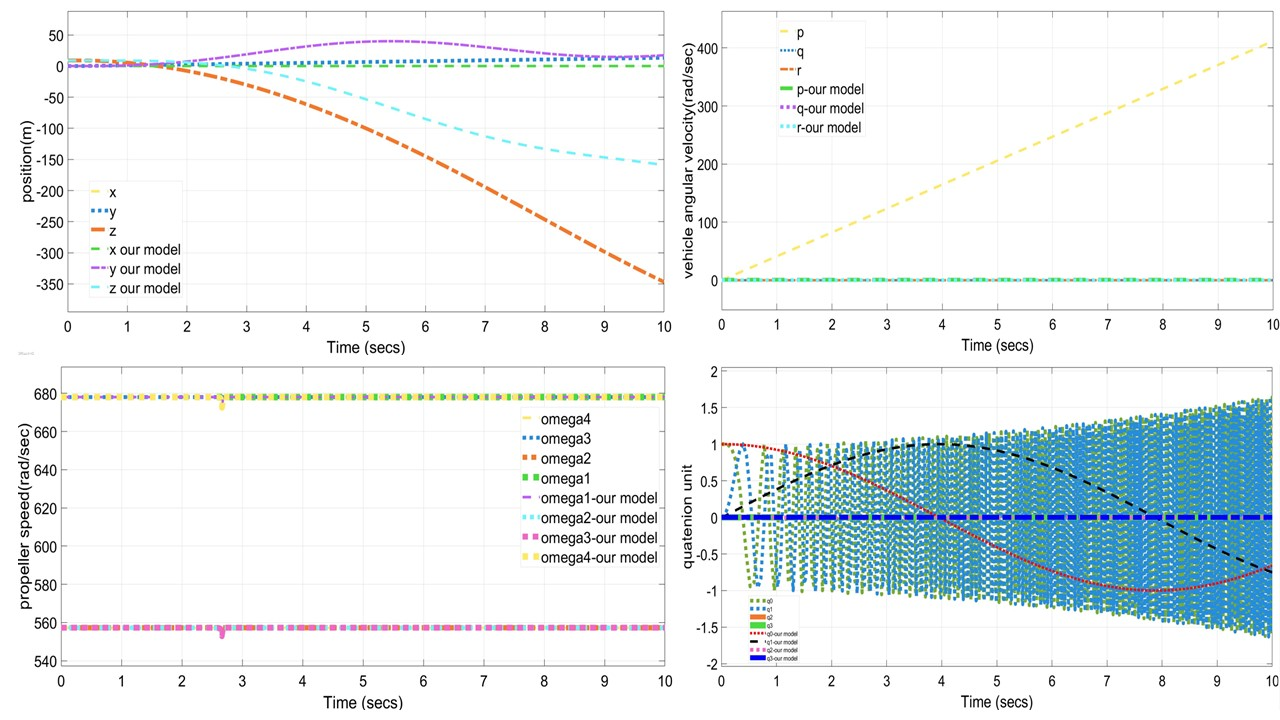
\includegraphics[width=1.0\linewidth]{figures/rollBest.jpg}
   % 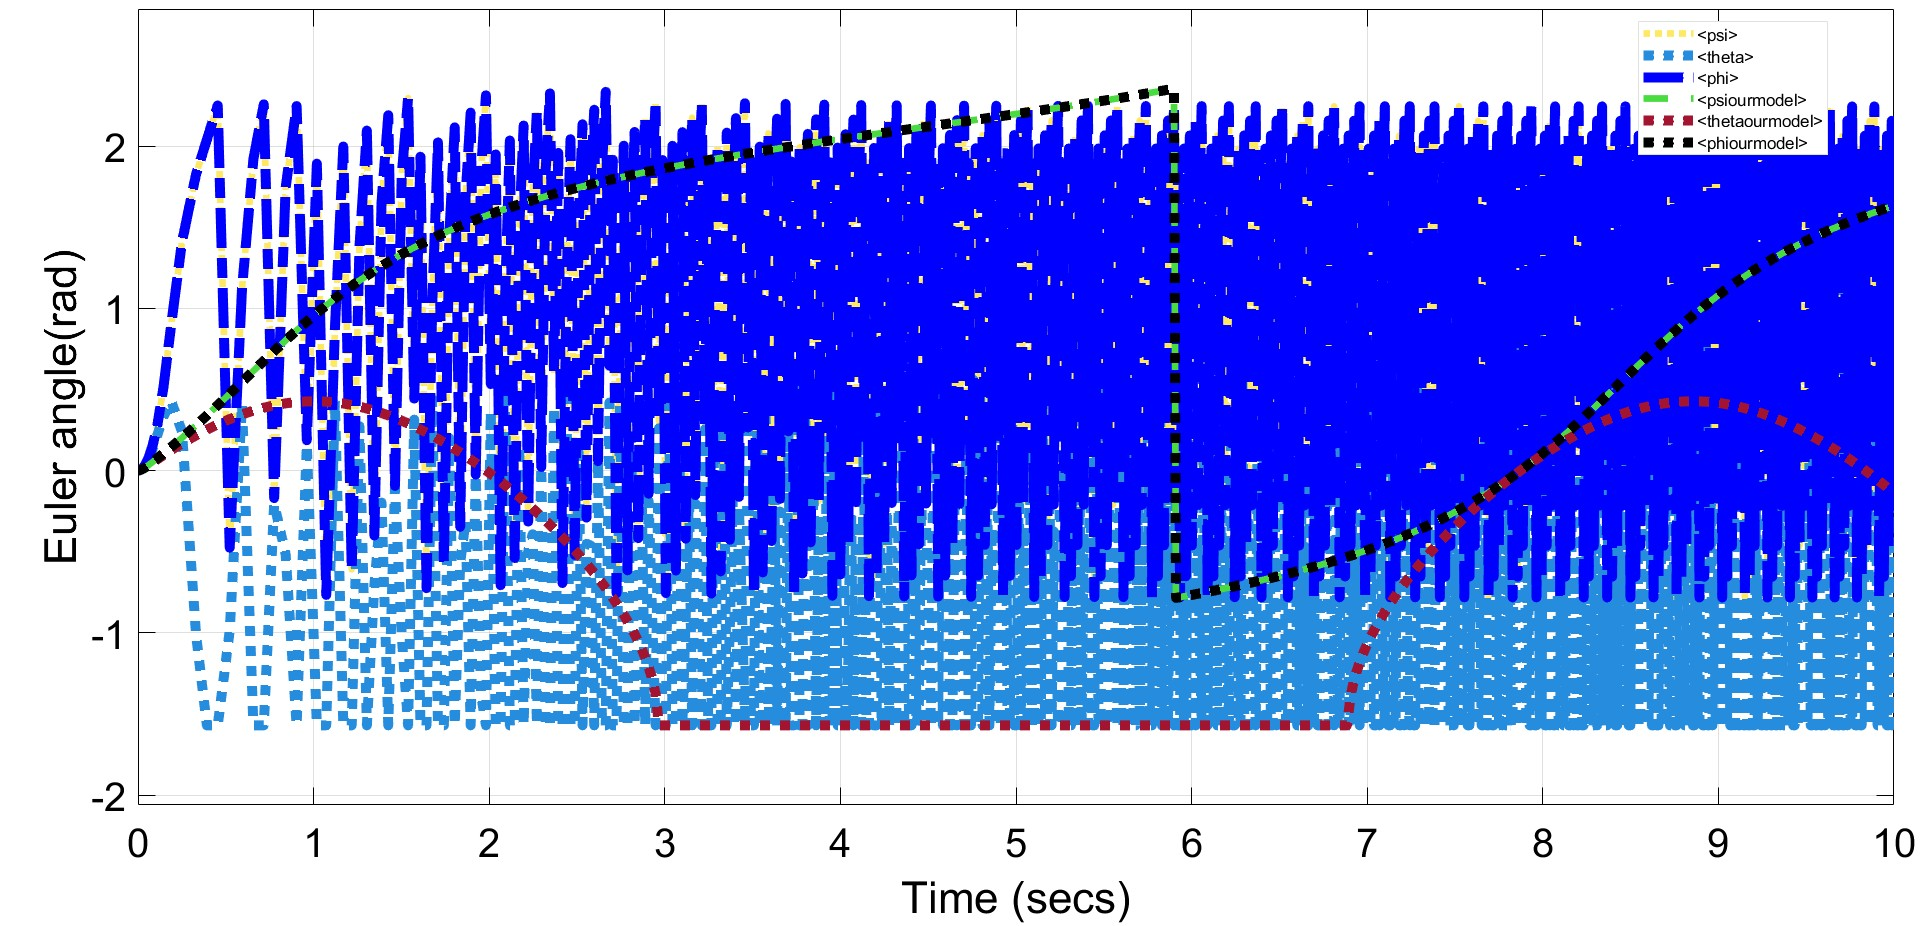
\includegraphics[width=1.0\linewidth]{figures/rolleuler.jpg}
   % \caption{Roll rotation due to $U_{1} = mg$ and $U_{2} = 0.2\,Nm$}
   % \label{fig:roll_rotation}
%\end{figure}

\begin{figure}[h!]
    \centering
    \begin{minipage}{0.48\linewidth}
        \centering
        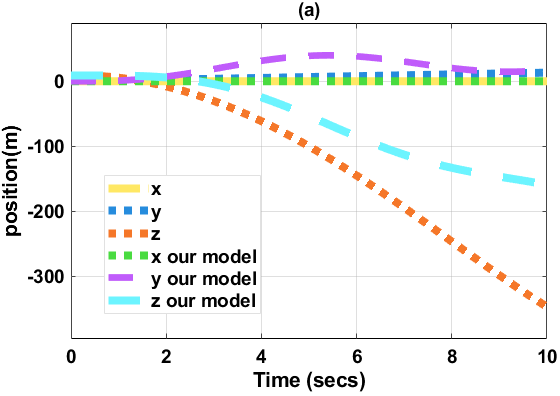
\includegraphics[width=1.0\linewidth]{figures/roll-position-BEST.png}
    \end{minipage}
    \hfill
    \begin{minipage}{0.48\linewidth}
        \centering
       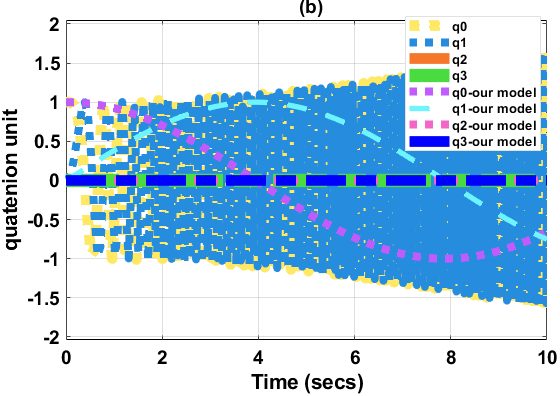
\includegraphics[width=1\linewidth]{figures/roll-quaternion-BEST.png}
    %\caption{Altitude controller diagram for maintaining desired quadrotor altitude}
    %\label{fig:attitude controller}
    \end{minipage}
\begin{minipage}{0.48\linewidth}
        \centering
        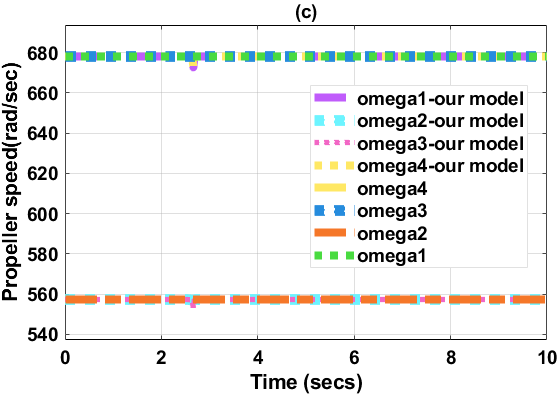
\includegraphics[width=1.0\linewidth]{figures/roll-propeller speed-BEST.png}
    \end{minipage}
    \begin{minipage}{0.48\linewidth}
        \centering
        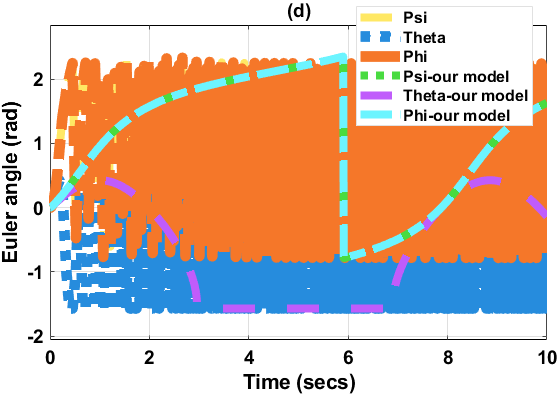
\includegraphics[width=1.0\linewidth]{figures/roll-euler-BEST.png}
    \end{minipage}
    \begin{minipage}{0.48\linewidth}
        \centering
        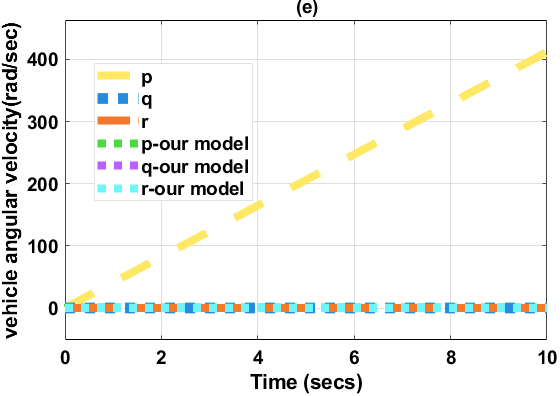
\includegraphics[width=1.0\linewidth]{figures/roll-vehicle speed-BEST.png}
    \end{minipage}
    \caption{Roll rotation due to $U_{1} = mg$ and $U_{2} = 0.2\,Nm$}
    \label{fig:roll_rotation}
\end{figure}


%\textbf{Pitch rotation} : At hovering, the pitch control torque is set to $U_{3}=0.2\,Nm$ while keeping $U_{1}$ constant. 
%This increases the speeds of motors 1 and 2 and decreases those of motors 3 and 4, 
%causing motion along the negative $x$-direction. Similar to roll, when the pitch angle 
%$\theta \geq \tfrac{\pi}{2}$, the quadrotor descends rapidly due to the combined effect 
%of thrust and gravity, as shown in Figure~\ref{fig:pitch_rotation}. 

%Using the canonical Euler triple, only pitch angles in the range $[-\tfrac{\pi}{2}, \tfrac{\pi}{2}]$ 
%are shown in the Euler-angle rotation graph. In contrast, the quaternion representation 
%allows rotation beyond this range without instability, demonstrating its singularity-free property.

\textbf{Pitch rotation} : At hovering, the pitch control torque is set to $U_{3}=0.2\,Nm$ while keeping $U_{1}$ constant.
Figure ~\ref{fig:pitch_rotation} illustrates the open-loop pitch response when a constant pitch torque is applied at hover. The position plots show a pronounced displacement in the longitudinal direction together with a rapid loss of altitude, confirming that once the vehicle pitches significantly, the thrust vector is no longer aligned with the vertical axis and can no longer fully balance weight. This effect develops faster in the baseline model, while the proposed model shows a slightly moderated fall due to aerodynamic drag. The propeller speeds separate into two steady groups, consistent with the control action required to generate pitching motion. The Euler-angle response indicates continuous growth of pitch, whereas roll and yaw remain close to zero. As expected, the quaternion states evolve smoothly beyond the Euler-angle range, confirming their suitability for representing large rotations without singularity. Similarly, the pitch-rate response increases steadily, while the other angular velocities remain small. Thus, the enhanced model captures pitch-induced instability more realistically.




%\begin{figure}[h!]
   % \centering
    %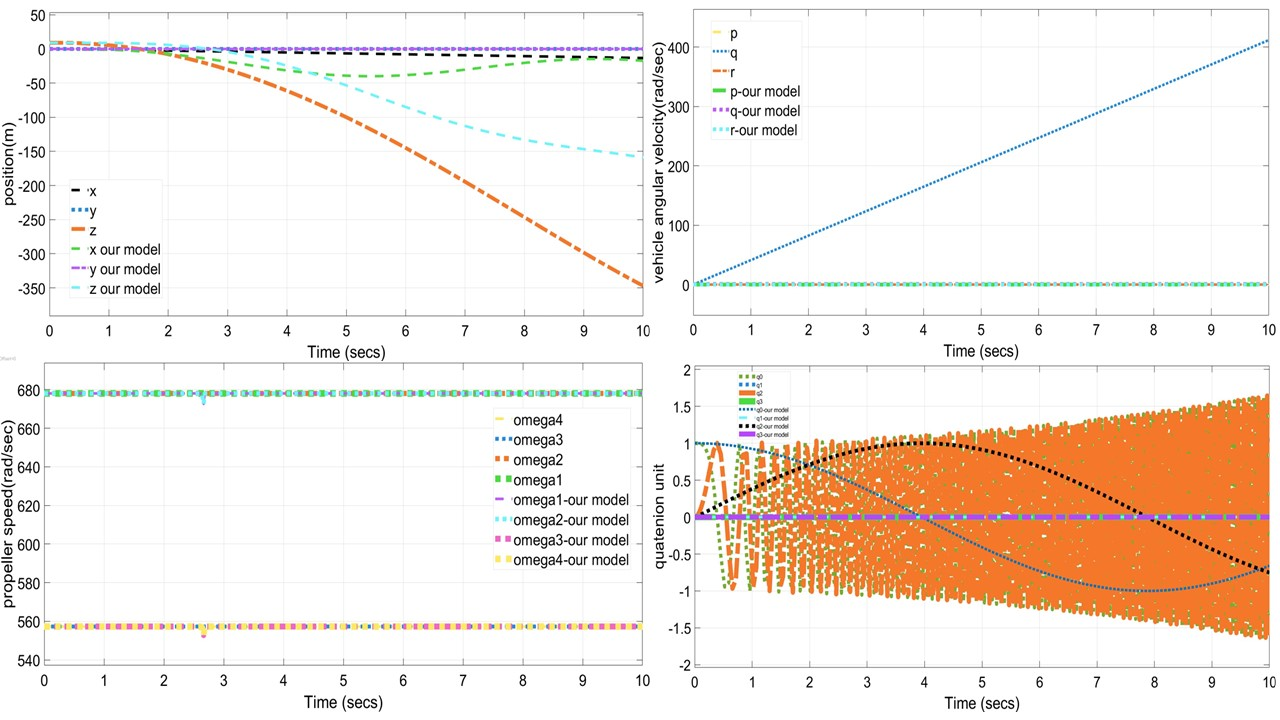
\includegraphics[width=1.0\linewidth]{figures/pitchBest.jpg}
   % 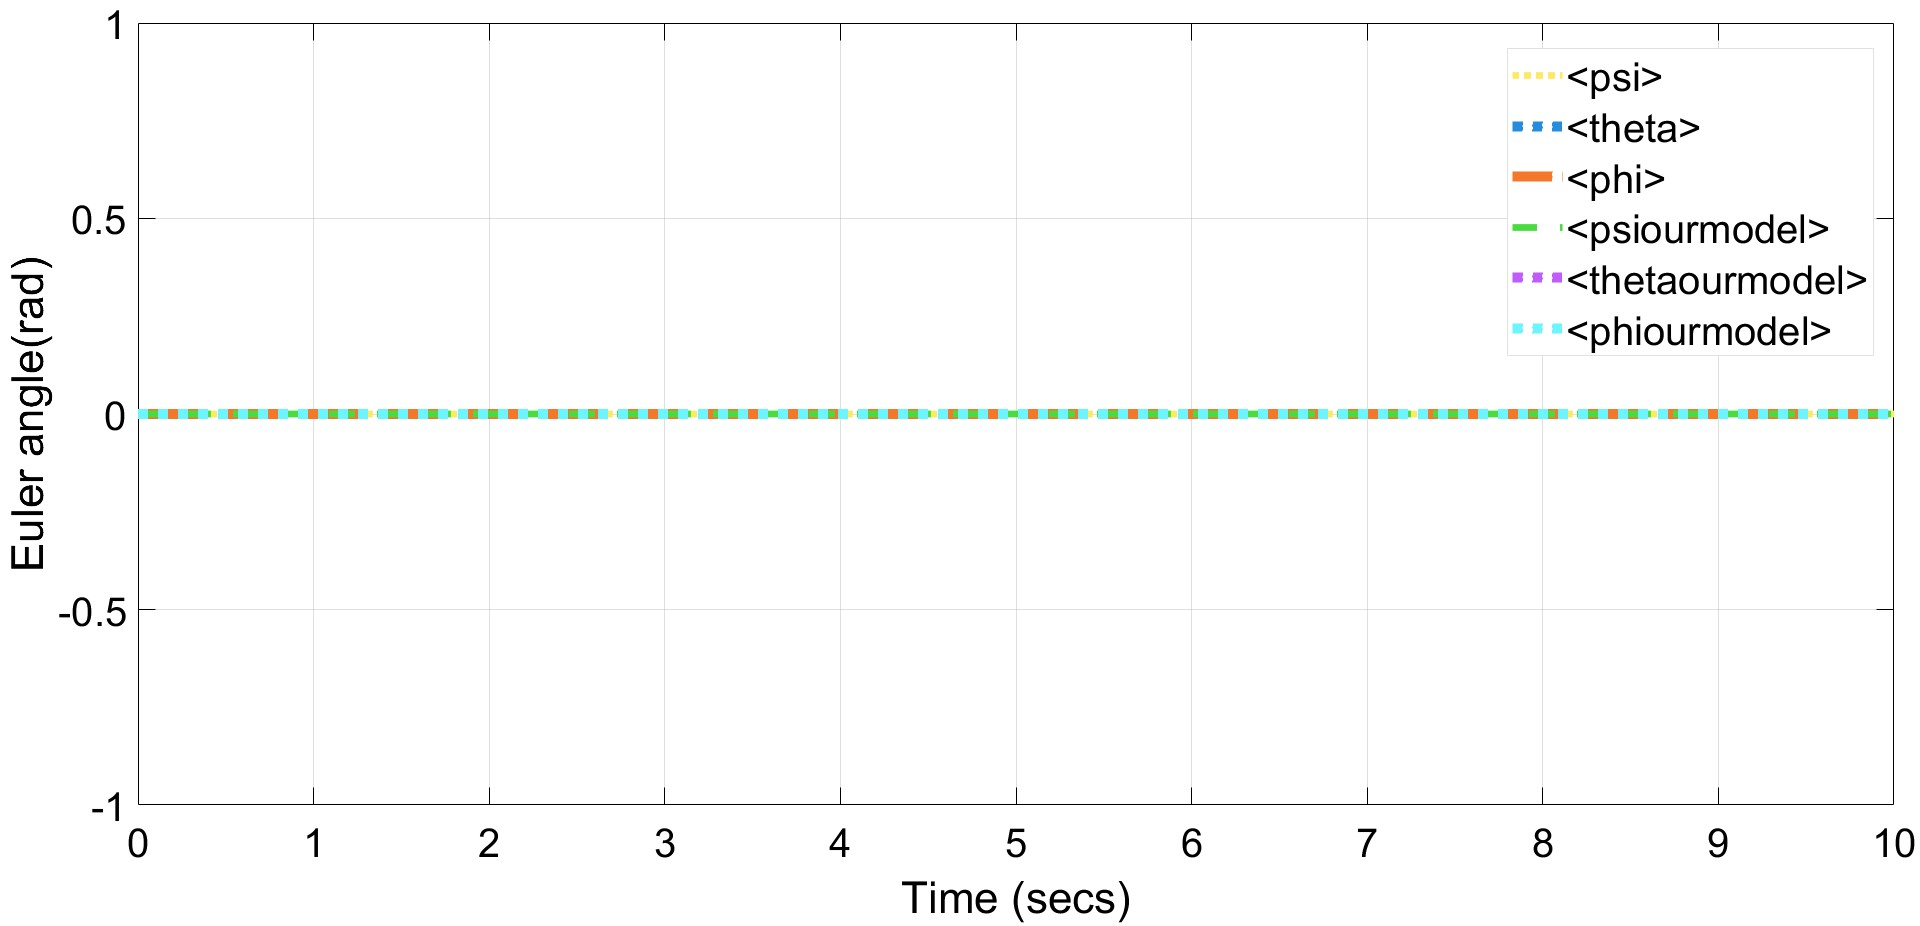
\includegraphics[width=1.0\linewidth]{figures/euleranglepitch.jpg}
    %\caption{Pitch rotation due to $U_{1} = mg$ and $U_{3} = 0.2\,Nm$}
    %\label{fig:pitch_rotation}
%\end{figure}

\begin{figure}[h!]
    \centering
    \begin{minipage}{0.48\linewidth}
        \centering
        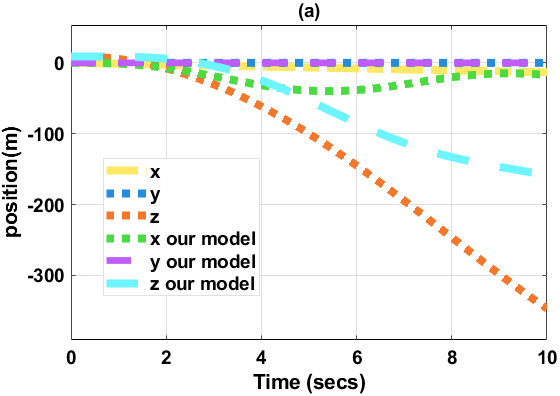
\includegraphics[width=1.0\linewidth]{figures/pitch-position-BEST.png}
    \end{minipage}
    \hfill
    \begin{minipage}{0.48\linewidth}
        \centering
       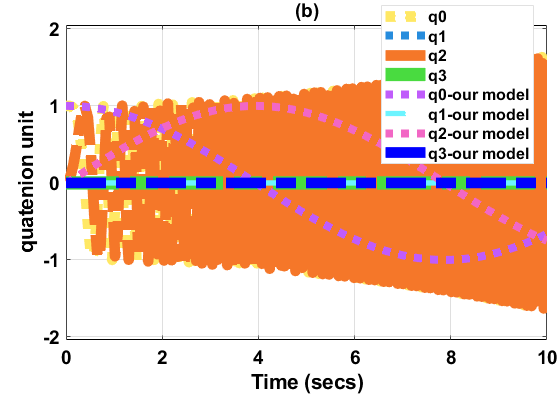
\includegraphics[width=1\linewidth]{figures/pitch-quaternion-BEST.png}
    %\caption{Altitude controller diagram for maintaining desired quadrotor altitude}
    %\label{fig:attitude controller}
    \end{minipage}
\begin{minipage}{0.48\linewidth}
        \centering
        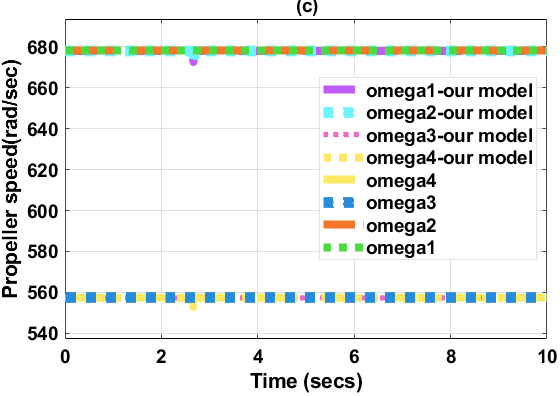
\includegraphics[width=1.0\linewidth]{figures/pitch-propeller speed-BEST.png}
    \end{minipage}
    \begin{minipage}{0.48\linewidth}
        \centering
        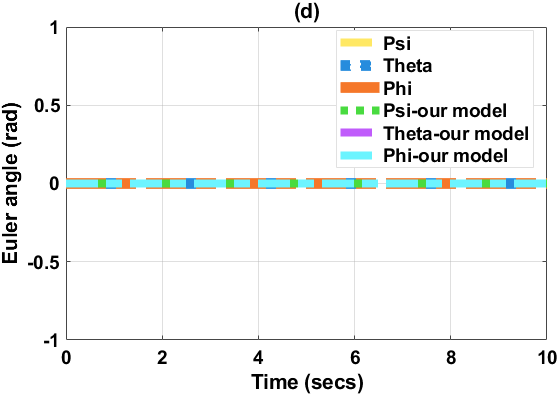
\includegraphics[width=1.0\linewidth]{figures/pitch-euler-BEST.png}
    \end{minipage}
    \begin{minipage}{0.48\linewidth}
        \centering
        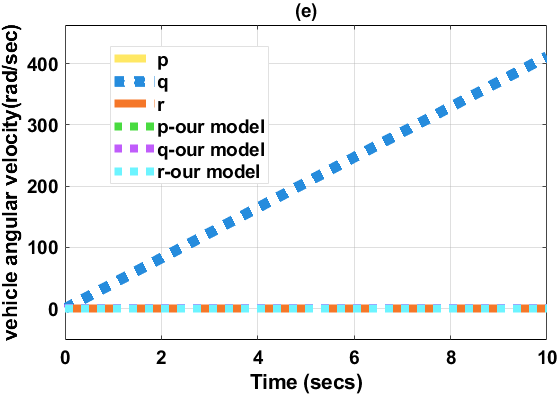
\includegraphics[width=1.0\linewidth]{figures/pitch-vehicle speed-BEST.png}
    \end{minipage}
    \caption{Pitch rotation due to $U_{1} = mg$ and $U_{3} = 0.2\,Nm$}
    \label{fig:pitch_rotation}
\end{figure}



%\textbf{The last scenario for Yaw rotation:} 
%At hovering, the yaw control torque is set to $U_{4} = 0.2\,Nm$, causing the quadrotor to rotate clockwise about the $z$-axis. This increases the speeds of motors 2 and 4 and decreases those of motors 1 and 3, while keeping $U_{1}$ (altitude) constant. No lateral motion along $x$ or $y$ occurs. By increasing the speed of propellers rotating in the same direction and decreasing the opposite ones, a net angular velocity is generated, resulting in a nonzero residual propeller speed $\Omega_r \neq 0$, as shown in Figure~\ref{fig:yaw_rotation}.

\textbf{The last scenario for Yaw rotation:} 
At hovering, the yaw control torque is set to $U_{4} = 0.2\,Nm$, causing the quadrotor 
to rotate clockwise about the $z$-axis. Figure ~\ref{fig:yaw_rotation} presents the yaw-rotation validation under a constant yaw torque while the total thrust is maintained at the hover condition. The position responses remain nearly constant, with altitude preserved around 9 m and no noticeable motion along the \(x\)- or \(y\)-axes, confirming that the applied input primarily excites rotational motion about the vertical axis. The propeller-speed plots show the expected split between counter-rotating motor pairs, which generates the required reaction torque for clockwise yaw. The Euler-angle response indicates that yaw evolves while roll and pitch remain essentially zero, confirming decoupled rotational behavior in this maneuver. The quaternion components vary consistently with pure heading rotation and remain bounded, showing smooth attitude representation throughout the motion. Similarly, the angular velocity response is dominated by the yaw rate, while roll and pitch rates stay close to zero. Overall, both models reproduce the expected yaw behavior, although the enhanced model remains more physically representative.


%\begin{itemize}
   % \item During roll and pitch maneuvers, propellers generate positive $U_2$ and $U_3$ 
   % for half the cycle and negative for the other half, producing back-and-forth 
   % lateral motion, as seen in Figures~\ref{fig:roll_rotation} and \ref{fig:pitch_rotation}.
    
   % \item Using the canonical Euler triple, roll and yaw angles in 
   % Figures~\ref{fig:roll_rotation} and \ref{fig:yaw_rotation} remain within 
   % $[-\pi, \pi]$.
%\end{itemize}

%The simulation results confirm that the derived quadrotor dynamic model behaves 
%as expected, validating its feasibility.
%Following this quantitative analysis, the next subsection focuses on the qualitative stability analysis at the operating point.

 %\begin{figure}[h!]
    % \centering
    %\includegraphics[width=0.6\textwidth]{your-yaw-figure.png} % insert figure here
    % 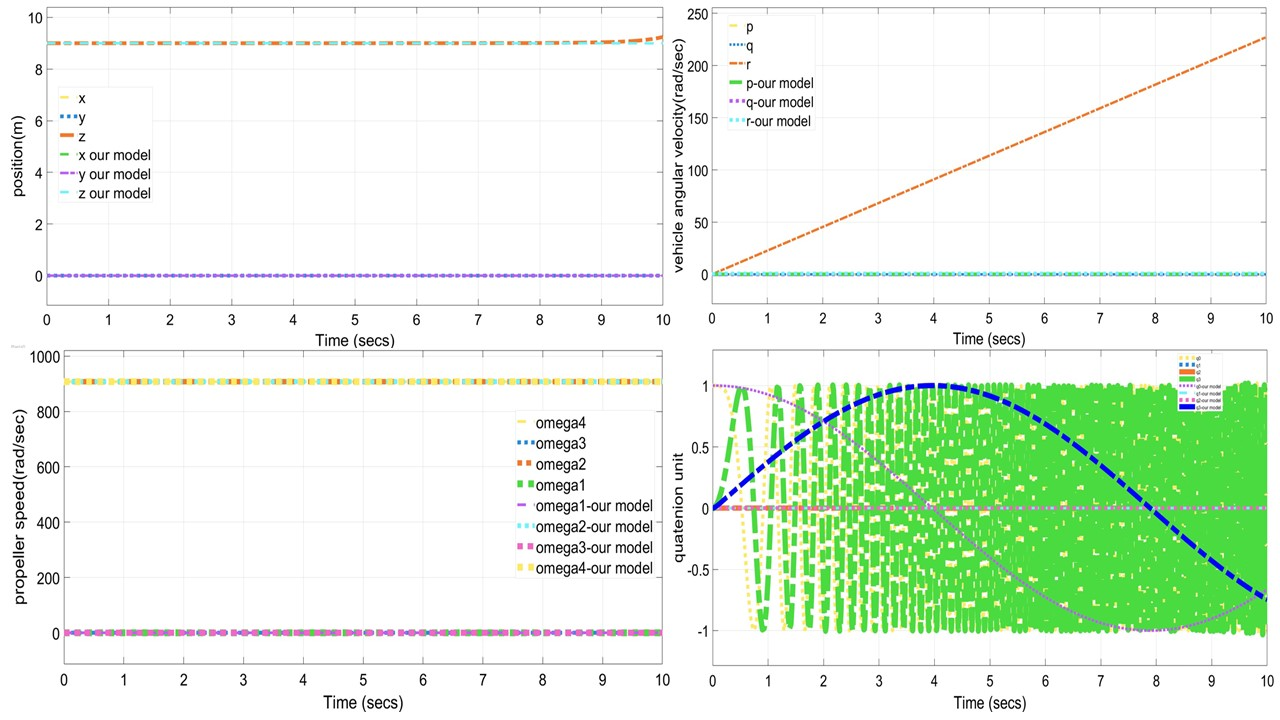
\includegraphics[width=1.0\linewidth]{figures/yawBest.jpg}
     %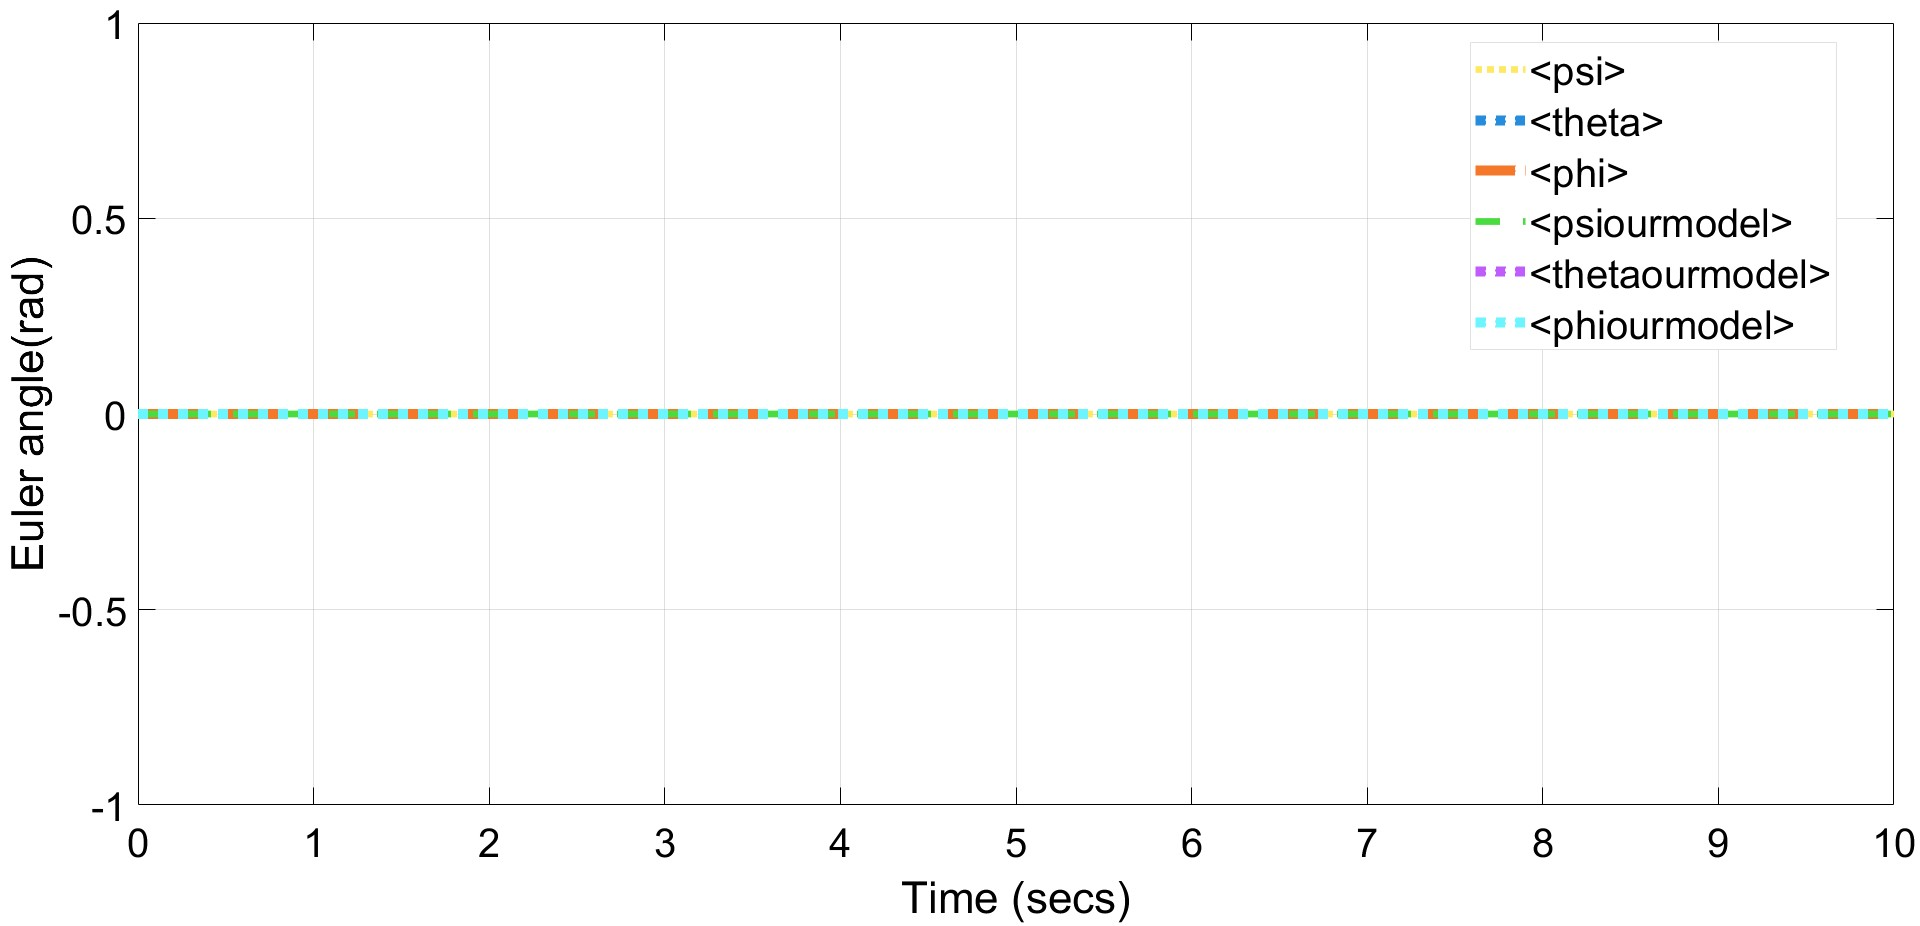
\includegraphics[width=1.0\linewidth]{figures/euleryaw.jpg}
     %\caption{CW yaw rotation due to $U_{1} = mg$ and $U_{4} = 0.2\,Nm$}
     %\label{fig:yaw_rotation}
 %\end{figure}

\begin{figure}[h!]
    \centering
    \begin{minipage}{0.48\linewidth}
        \centering
        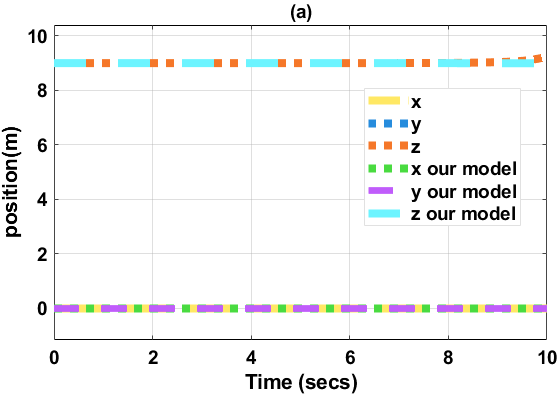
\includegraphics[width=1.0\linewidth]{figures/yaw-position-BEST.png}
    \end{minipage}
    \hfill
    \begin{minipage}{0.48\linewidth}
        \centering
       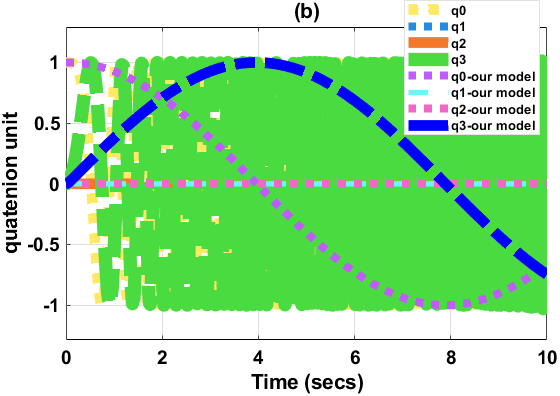
\includegraphics[width=1\linewidth]{figures/yaw-quaternion-BEST.png}
    %\caption{Altitude controller diagram for maintaining desired quadrotor altitude}
    %\label{fig:attitude controller}
    \end{minipage}
\begin{minipage}{0.48\linewidth}
        \centering
        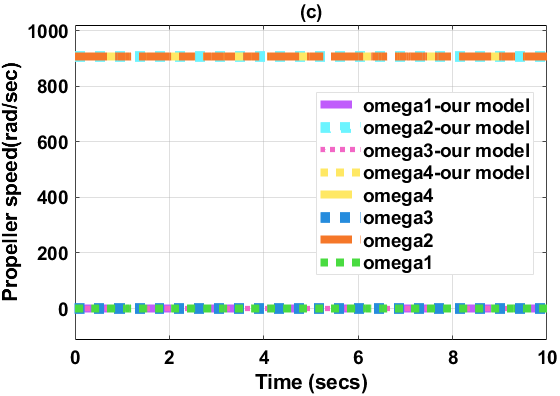
\includegraphics[width=1.0\linewidth]{figures/yaw-propeller speed-BEST.png}
    \end{minipage}
    \begin{minipage}{0.48\linewidth}
        \centering
        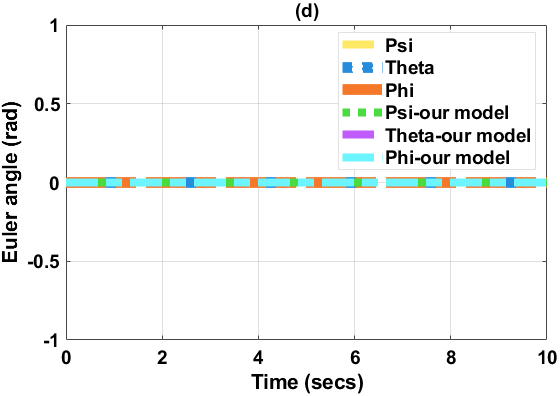
\includegraphics[width=1.0\linewidth]{figures/yaw-euler-BEST.png}
    \end{minipage}
    \begin{minipage}{0.48\linewidth}
        \centering
        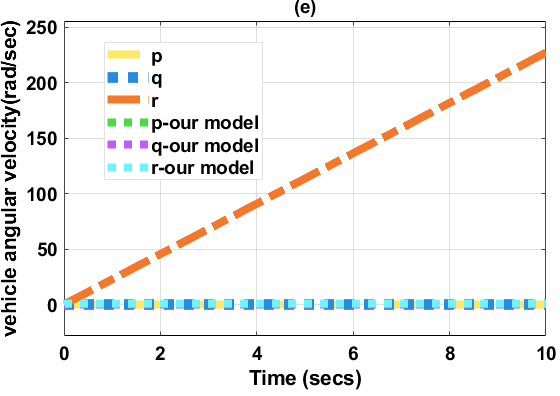
\includegraphics[width=1.0\linewidth]{figures/yaw-vehicle speed-BEST.png}
    \end{minipage}
    \caption{CW yaw rotation due to $U_{1} = mg$ and $U_{4} = 0.2\,Nm$}
    \label{fig:yaw_rotation}
\end{figure}


\begin{table}[htbp]
\centering
\caption{PSO Performance for Different Numbers of Particles in Attitude Gains Tuning}
\label{tab:PSO_ITAE_attitude}

\resizebox{\linewidth}{!}{%
\begin{tabular}{|c|c|c|c|c|}
\hline
\textbf{Nop} & \textbf{max. iteration} & \textbf{Time (minutes)} &
\textbf{1st iteration GBEST} & \textbf{100th iteration GBEST (\% improvement)} \\ \hline
15 & 100 & 30  & 10.0610 & 7.1602 (28.83\%) \\ \hline
30 & 100 & 86  & 9.0872  & 7.6509 (15.81\%) \\ \hline
45 & 100 & 105 & 8.9855  & 7.5439 (16.04\%) \\ \hline
60 & 100 & 136 & 8.4118  & 7.2328 (14.02\%) \\ \hline
75 & 100 & 167 & 9.2651  & 7.6608 (17.31\%) \\ \hline
\end{tabular}
}%
\end{table}


\begin{table}[htbp]
\centering

\caption{PSO Performance for Different Numbers of Particles in Position Gains Tuning}
\label{tab:PSO_Position_Gains}

\resizebox{\linewidth}{!}{%
\begin{tabular}{|c|c|c|c|c|}
\hline
\textbf{Nop} & \textbf{Max. Iteration} & \textbf{Time (minutes)} &
\textbf{1st iteration GBEST} & \textbf{100th iteration GBEST (\% improvement)} \\ \hline

15 & 100 & 38  & 64.1658 & 63.1375 (1.60\%) \\ \hline
30 & 100 & 60  & 70.6404 & 63.1375 (10.63\%) \\ \hline
45 & 100 & 67  & 63.6148 & 63.1375 (0.75\%) \\ \hline
60 & 100 & 93  & 63.5962 & 63.1375 (0.72\%) \\ \hline
75 & 100 & 105 & 63.5222 & 63.1375 (0.61\%) \\ \hline

\end{tabular}
}
\end{table}

\section{PSO tunning results}
%Below figure shows how ITAE values were changing with respect to number of particle swarm size  during attitude and position controller gains optimization see Fig.\ref{fig:Attitude ITAE} and Fig.\ref{fig:Position ITAE}%

The results in Tables \ref{tab:PSO_ITAE_attitude} and \ref{tab:PSO_Position_Gains}, together with  Fig.\ref{fig:Attitude ITAE} and Fig.\ref{fig:Position ITAE}, demonstrate the effectiveness of PSO in tuning the ASTSMC gains. For attitude control, a clear reduction in ITAE is observed across all particle sizes, with faster convergence achieved at lower swarm sizes, particularly Number of Particles (Nop) = 15, indicating computational efficiency without compromising performance. In contrast, position control shows minimal variation in final ITAE values, as all configurations converge to a similar optimum, suggesting a well-defined solution space. Increasing particle size mainly affects convergence behavior rather than final performance. Thus, PSO provides consistent and reliable tuning for both attitude and position dynamics.

\begin{figure}[h!]
    \centering
    \begin{minipage}{0.48\linewidth}
        \centering
        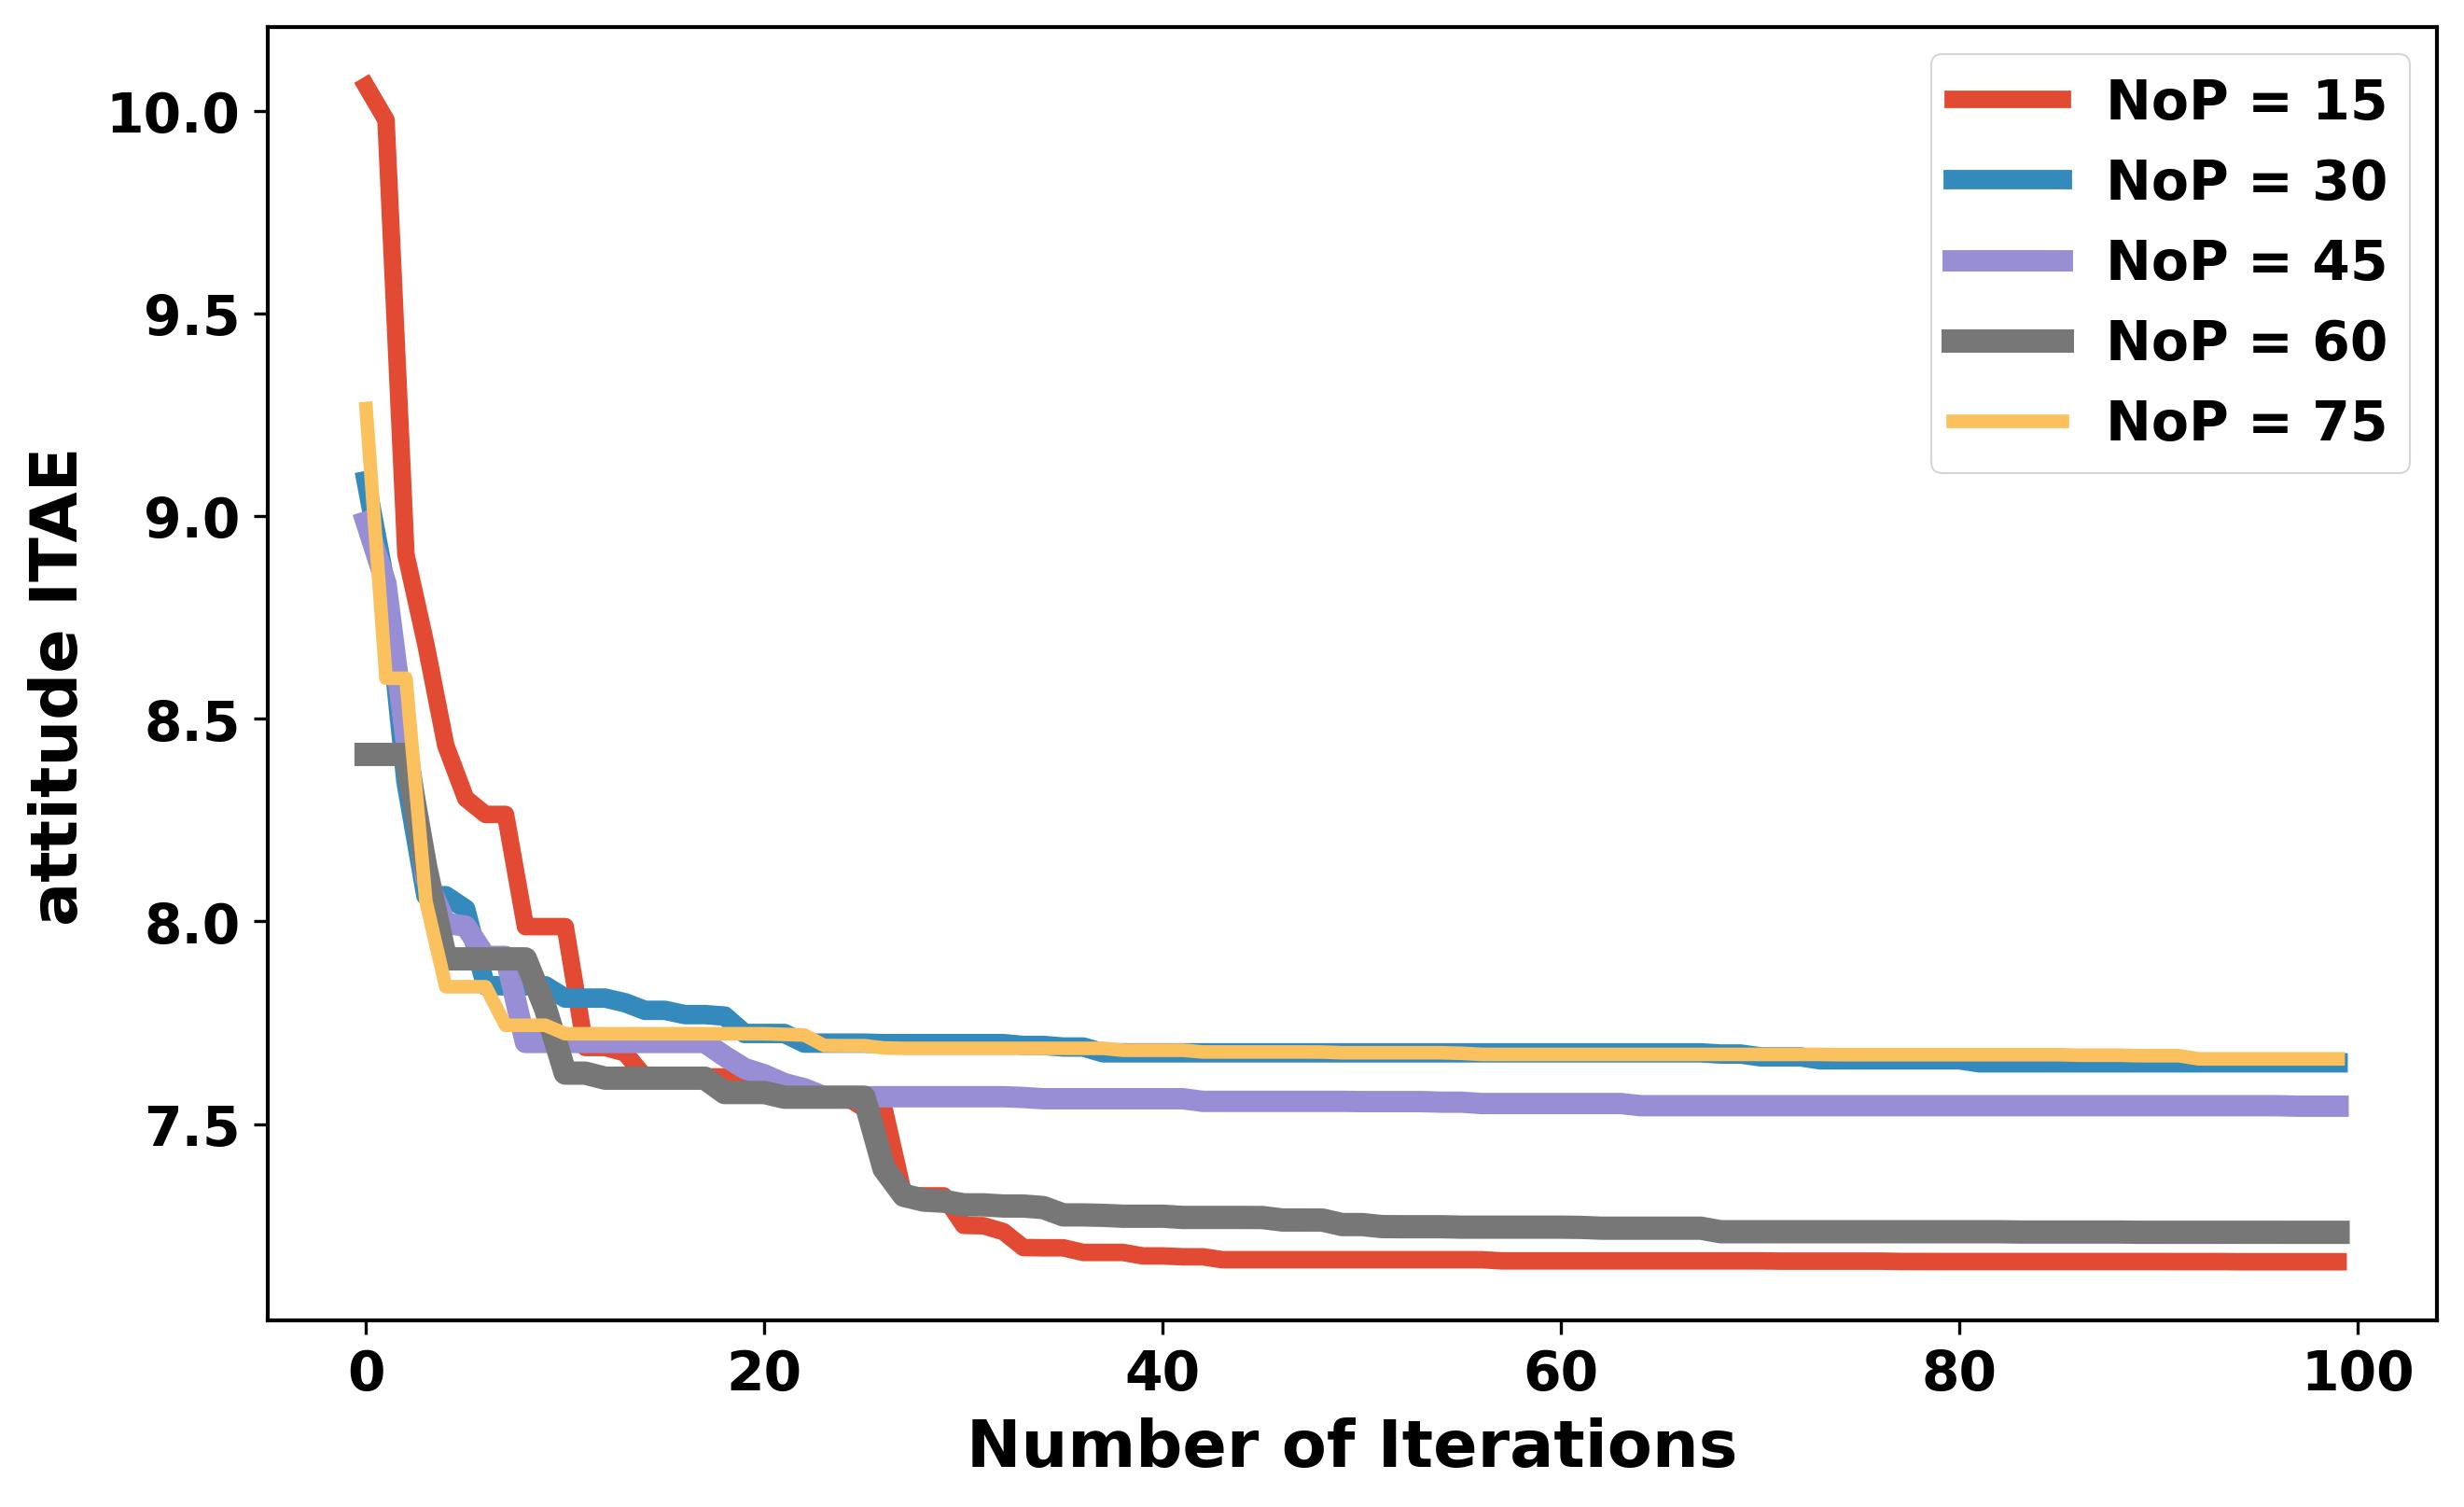
\includegraphics[width=\linewidth]{figures/attitude ITAE_plot.jpg}
        \caption{Attitude ITAE against Number of Iterations for different Particle Swarm Size}
        \label{fig:Attitude ITAE}
    \end{minipage}
    \hfill
    \begin{minipage}{0.48\linewidth}
        \centering
        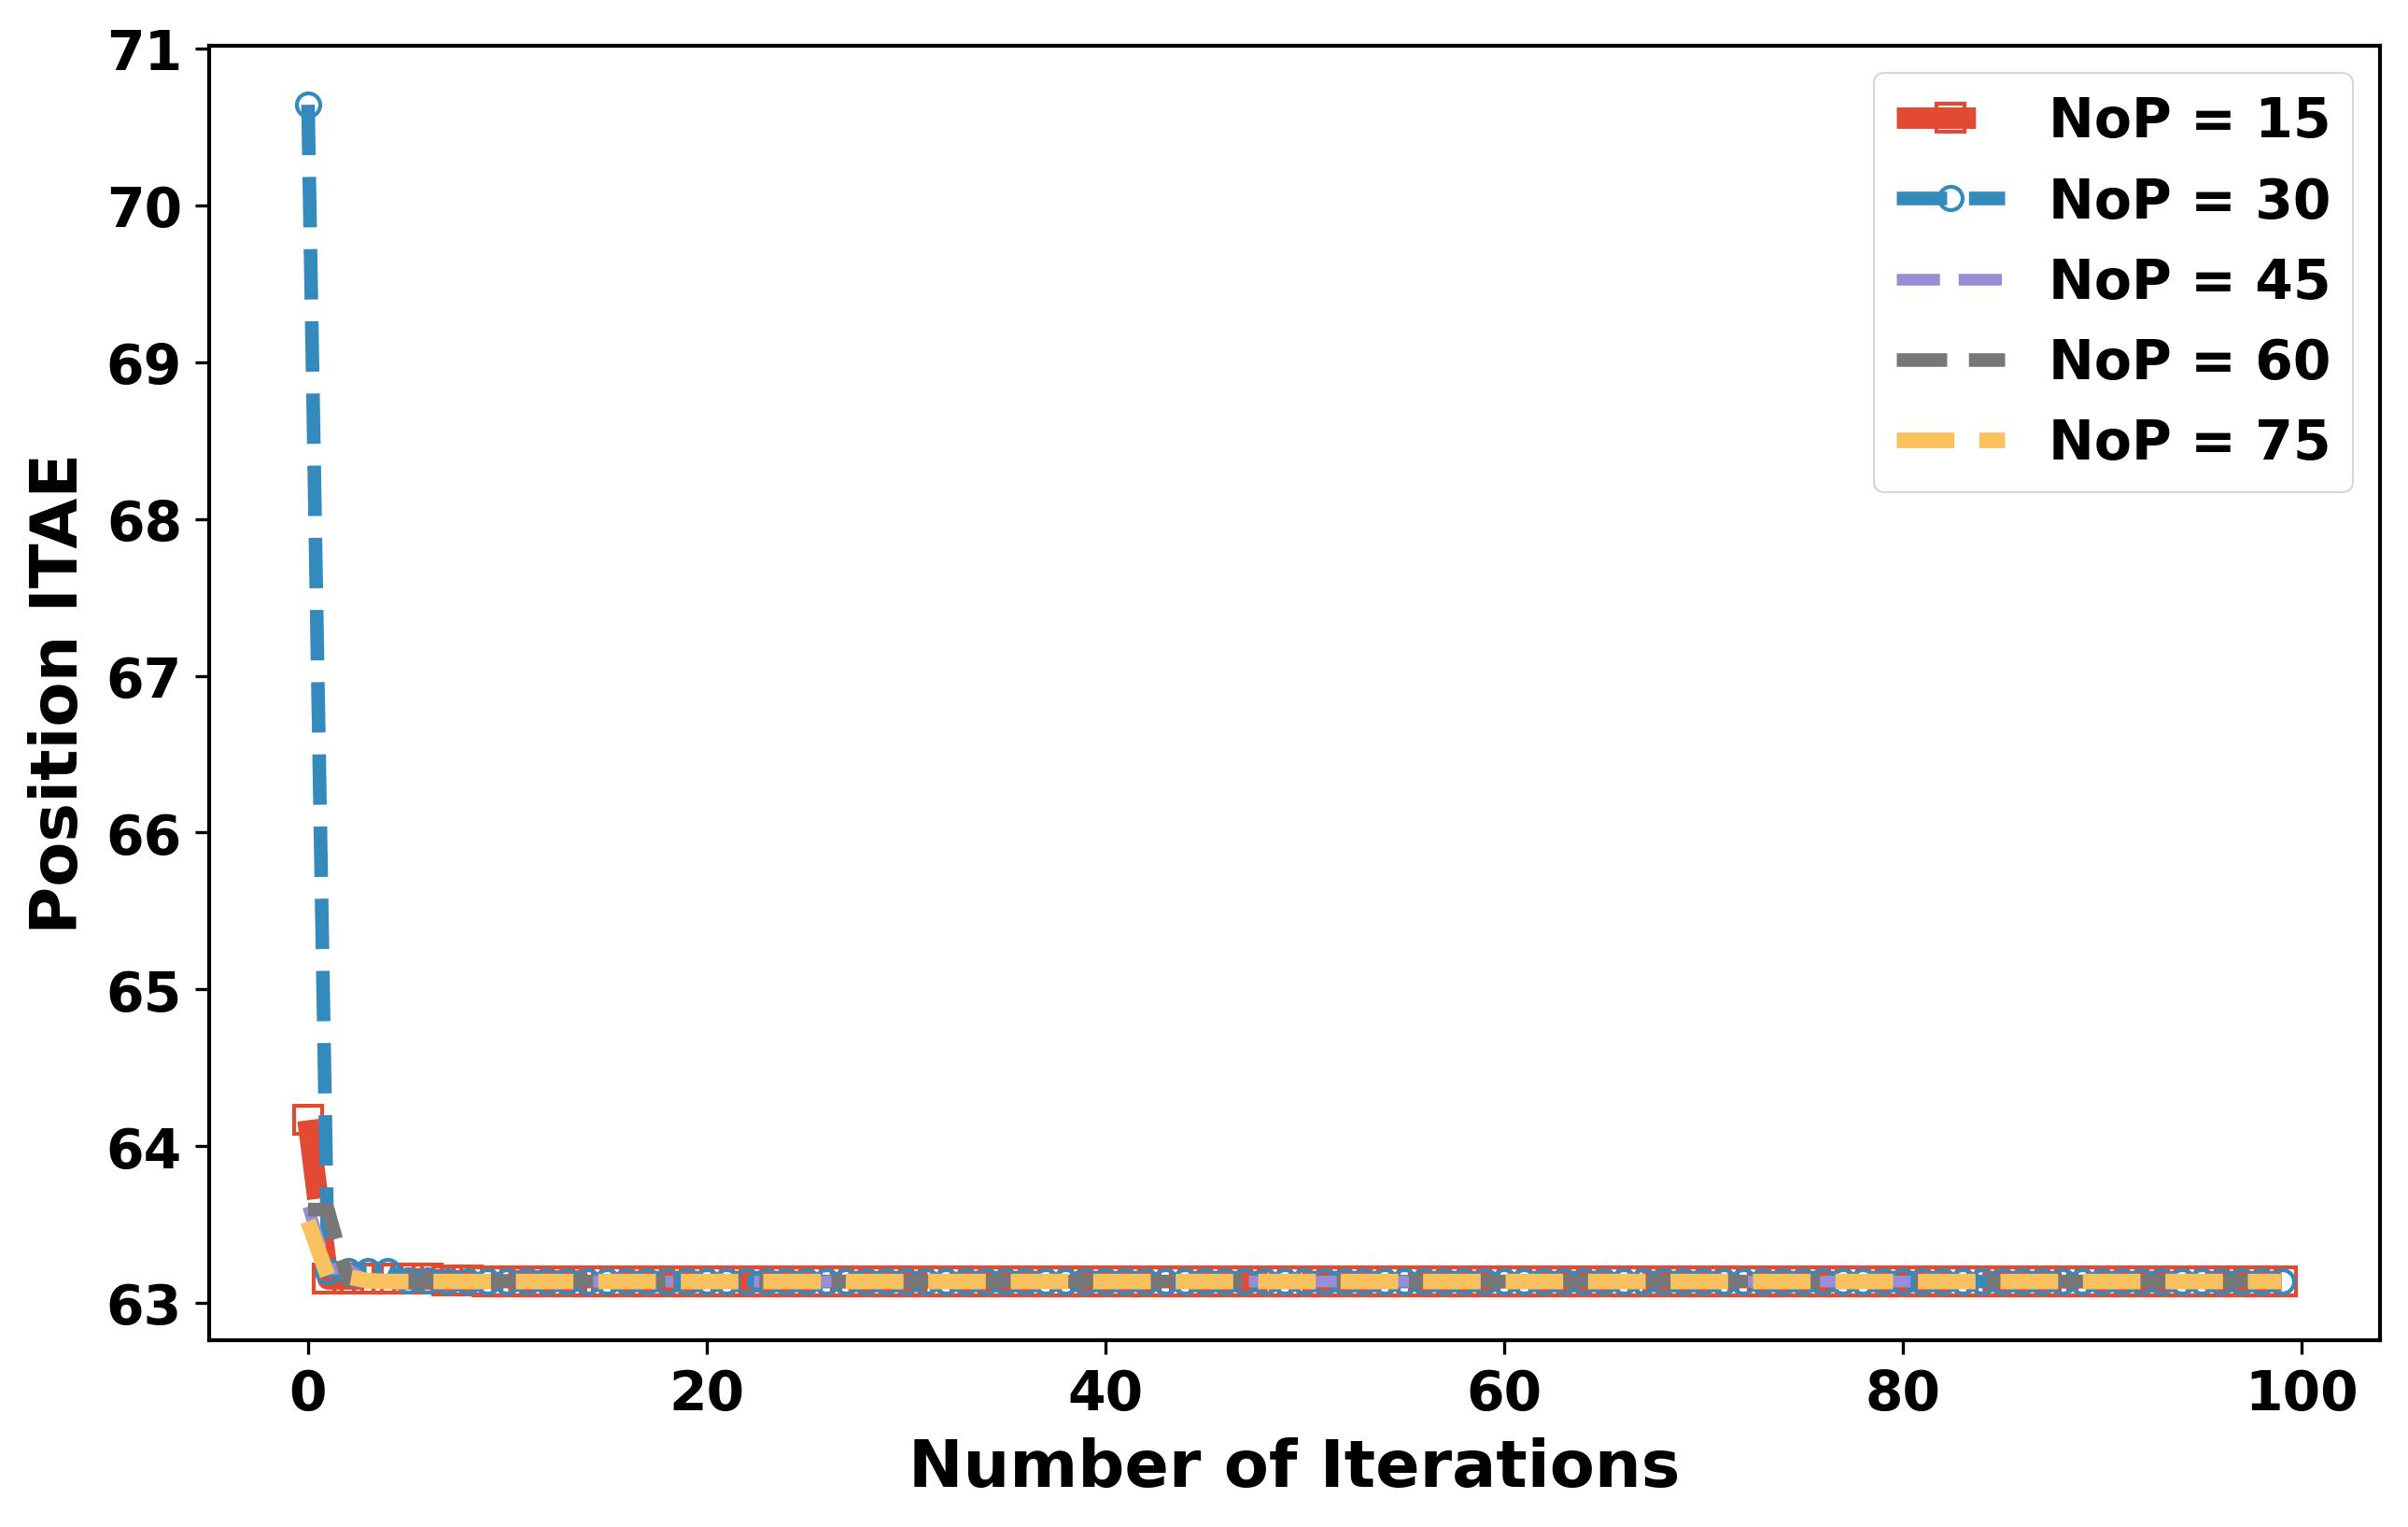
\includegraphics[width=\linewidth]{figures/position ITAE_plot.jpg}
        \caption{Position ITAE against Number of Iterations for different Particle Swarm Size}
        \label{fig:Position ITAE}
    \end{minipage}
\end{figure}

%\begin{figure}[h!]
   %\ \centering
    %\
\includegraphics[width=0.85\linewidth]{Figures/attitude ITAE_plot.jpg}
    %\\caption{Attitude ITAE against Number of Iterations for different Particle Swarm Size}
    %\\label{fig:Attitude ITAE}
%\\end{figure}

%\\begin{figure}[h!]
   %\ \centering
   %\ 
\includegraphics[width=0.85\linewidth]{Figures/position ITAE_plot.jpg}
   %\ \caption{Position ITAE against Number of Iterations for different Particle Swarm Size}
    %\\label{fig:Position ITAE}
%\\end{figure}





\section{Trajectory Tracking Results}
The simulation of designed quadcopter model was done in Matlab/Simulink environment. 
The quadcopter parameter used in the simulation is as shown in Table\ref{tab:Plant parameter for simulation}. 
Simulation results created using Simulink give an insight about performance of the designed controller, 
the controller’s initial gains were initially tuned using a particle swarm optimization (PSO) approach, 
then after controller gains were being tuned in real time by adaptive laws of adaptive super twisting 
sliding mode controller. Designed controller was tested in handling parameter variations and disturbances 
without failing to track desired trajectories, then after spiral infinity and ramp helix trajectory tracking was done to check its ability to follow desired trajectory. During all these simulations the performance of it was 
compared to back stepping sliding mode controller (BSMC) \cite{bouadi2007sliding} and conventional PID.

\subsection{ Parameter variation handling capacity}

To demonstrate efficiency and robustness of the designed controller in tracking the desired trajectories 
under parameter variations, following desired trajectories were used:
\begin{equation}
x_d = 1 - \cos(t), \quad y_d = \sin(t), \quad z_d = t, \quad \psi_d = 0
\end{equation}

Mass of quadcopter was increased from 1kg to 1.5kg for the whole period of simulation, this indicate an 
addition of 0.5kg equivalent to 50\% in quadcopter’s mass, inertias along $x$, $y$ and $z$ axis were kept 
constant. With reference to Figures \ref{fig:x tracking with parametric variation}--\ref{fig:yaw tracking with parametric variation}, Figures \ref{fig:U1 parametric variation}--\ref{fig:U4 parametric variation} and Table\ref{ITAE for parametric variation}, following insight were realized.

% With reference to Figs\ref{fig:x tracking with parametric variation},\ref{fig:y tracking with parametric variation},\ref{fig:z tracking with parametric variation},  \ref{fig:yaw tracking with parametric variation}, \ref{fig:U1 parametric variation},\ref{fig:U2 parametric variation},\ref{fig:U3 parametric variation},\ref{fig:U4 parametric variation} and Table\ref{ITAE for parametric variation}, following insight were realized.

An adaptive super twisting sliding mode controller (ASTSMC) demonstrates remarkable parametric robustness 
with only 58\% degradation in X-tracking and 2\% in Y-tracking compared to back stepping sliding mode 
control (BSMC) catastrophic 97\% Y-axis failure under 50\% mass uncertainty. This 48.5 times improvement 
in Y-tracking validates the adaptive super twisting mechanism's ability to compensate model mismatches 
in real time. While PID achieves superior X-axis performance (40\% degradation), it suffers 21\% Z-axis 
deterioration versus ASTSMC's exceptional 79\% Z-tracking retention. The 100\% yaw error in ASTSMC 
indicates conservative tuning prioritizing position control over orientation an acceptable tradeoff for 
trajectory tracking missions. ASTSMC achieves 65\% reduction in thrust demand ($U_1$) compared to PID's 
36\%, demonstrating superior energy efficiency critical for battery powered UAVs. The adaptive gains 
maintain $U_2$, $U_3$, $U_4$ torques at 47\%, 15\%, and 100\% of nominal values, avoiding actuator 
saturation while BSMC demands 52--61\% torque increases, risking hardware limits. An adaptive super 
twisting sliding mode controller’s adaptive nature ensures parametric invariance with minimal control 
expenditure, outperforming fixed gain controllers by simultaneously achieving tracking accuracy and 
energy optimization essential for robust autonomous flight under model uncertainties.

%\begin{figure}
   % \centering
    %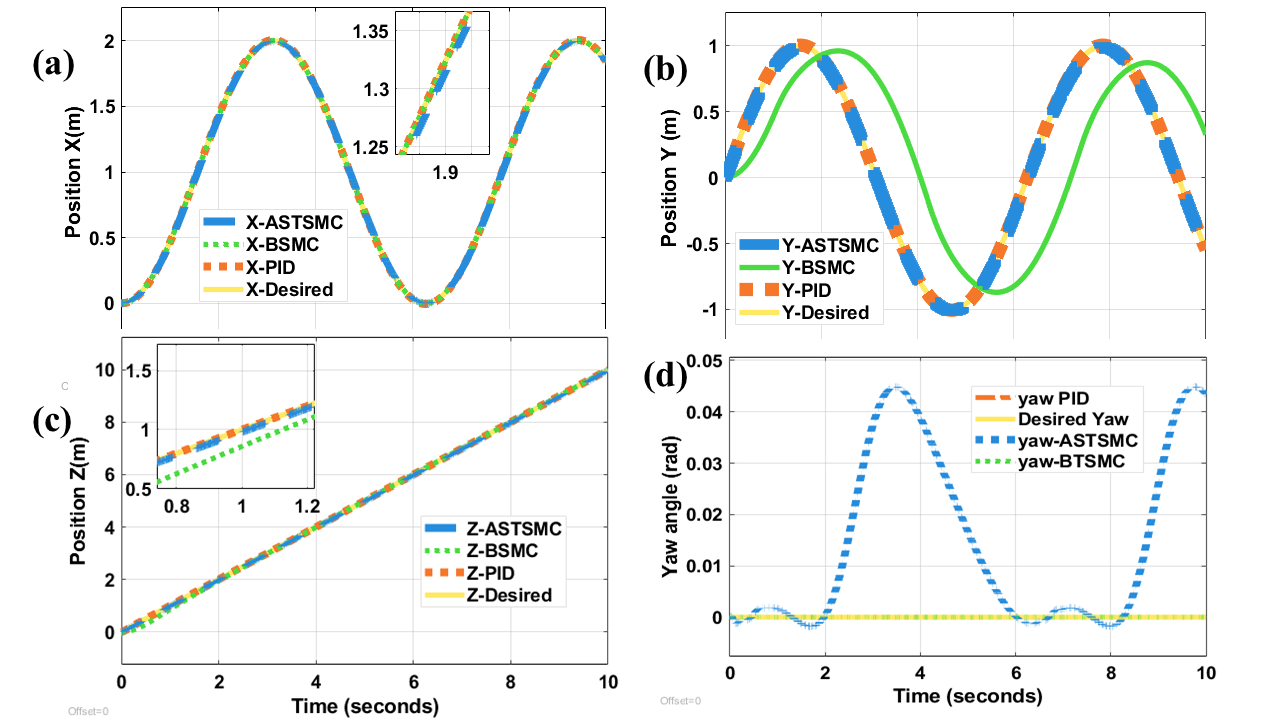
\includegraphics[width=1\linewidth]{figures/position tracking parametric variation.png}
   % \caption{Position trajectory tracking $a,b,c$  and yaw tracking $d$ during parametric variation handling}
   % \label{fig:position parametric variation handling}
%\end{figure}

%\begin{figure}
   % \centering
    %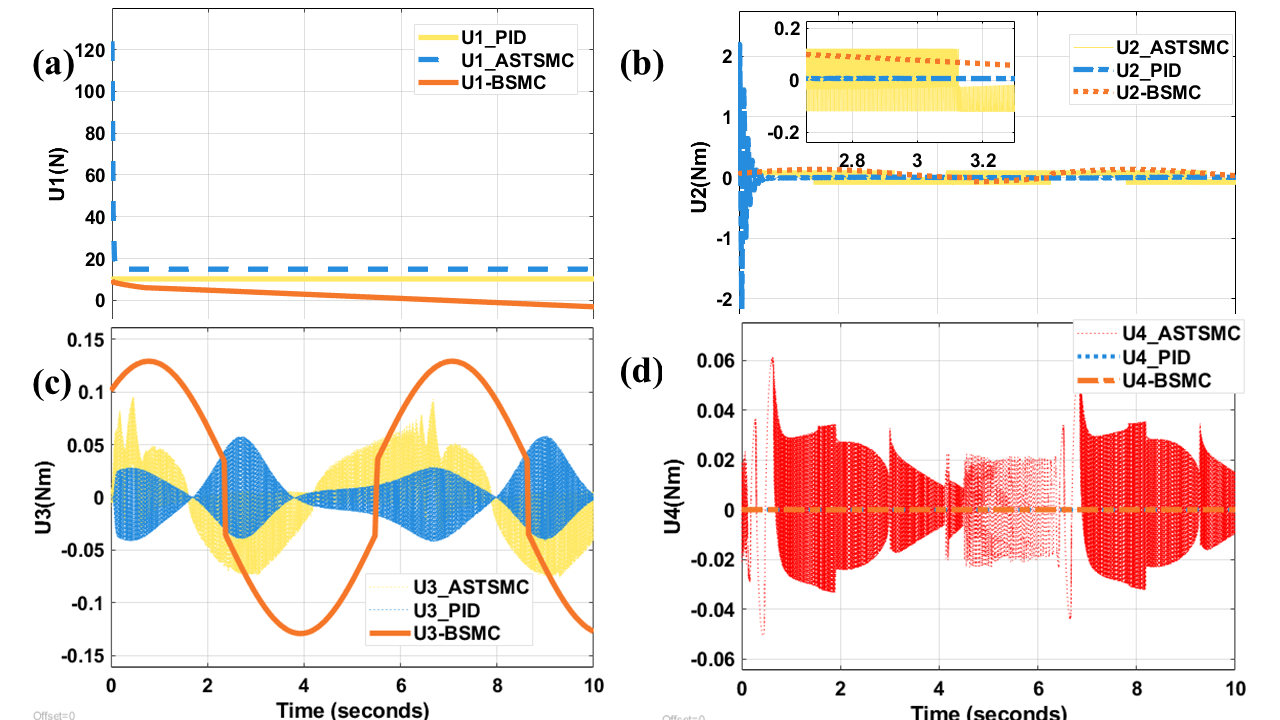
\includegraphics[width=1\linewidth]{figures/control inputs with parametric variations.png}
    %\caption{Control inputs $a,b,c$  and  $d$ during parametric variation handling}
    %\label{fig:control inputs for parametric variation handling}
%\end{figure}
%%%%%%%%%%%%%%%%%%%%%%%%%%%%%%%%%%%%%%%%%%%%%%%%%%%%%%%%
\begin{figure}[h!]
    \centering
    \begin{minipage}{0.48\linewidth}
        \centering
        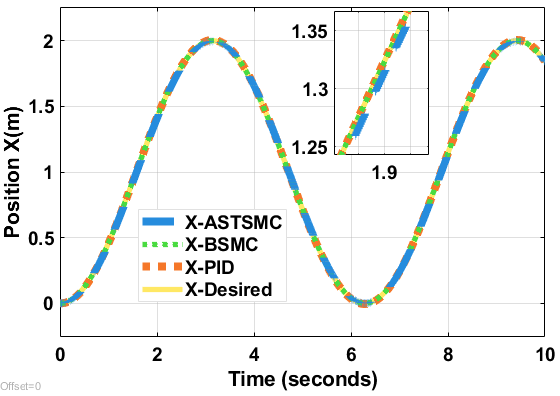
\includegraphics[width=\linewidth]{figures/x-tracking parametric variation.png}
        \caption{Position X tracking with parametric variation}
        \label{fig:x tracking with parametric variation}
    \end{minipage}
    \hfill
    \begin{minipage}{0.48\linewidth}
        \centering
        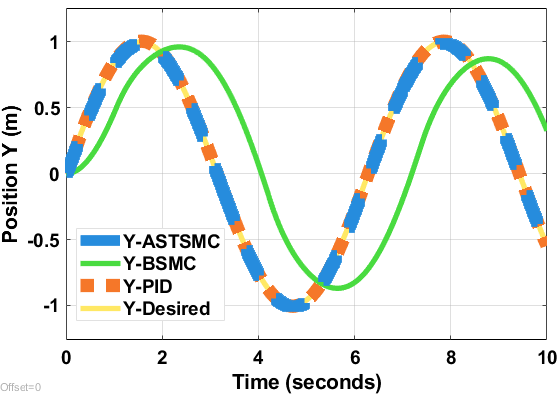
\includegraphics[width=\linewidth]{figures/y-tracking parametric variation.png}
        \caption{Position Y tracking with parametric variation}
        \label{fig:y tracking with parametric variation}
    \end{minipage}
%\end{figure}

  \hfill
    \begin{minipage}{0.48\linewidth}
        \centering
        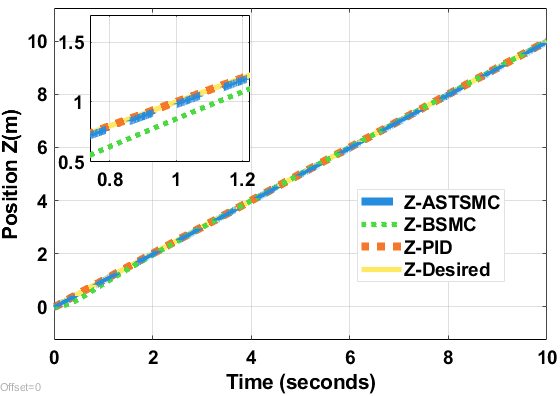
\includegraphics[width=\linewidth]{figures/z-tracking parametric variation.png}
        \caption{Position Z tracking with parametric variation}
        \label{fig:z tracking with parametric variation}
    \end{minipage}
%\end{figure}
  \hfill
    \begin{minipage}{0.48\linewidth}
        \centering
        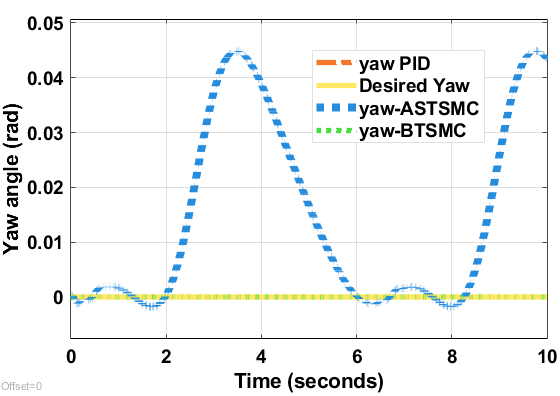
\includegraphics[width=\linewidth]{figures/yaw-tracking parametric variation.png}
        \caption{Yaw tracking with parametric variation}
        \label{fig:yaw tracking with parametric variation}
    \end{minipage}
\end{figure}




\begin{figure}[h!]
    \centering
    \begin{minipage}{0.48\linewidth}
        \centering
        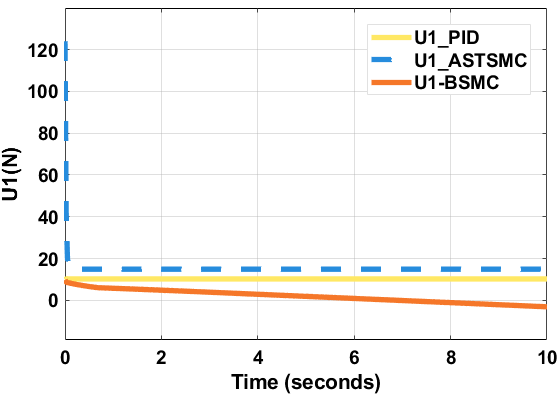
\includegraphics[width=\linewidth]{figures/U1-for parametric variation.png}
        \caption{Control input U1 during parametric variation}
        \label{fig:U1 parametric variation}
    \end{minipage}
    \hfill
    \begin{minipage}{0.48\linewidth}
        \centering
        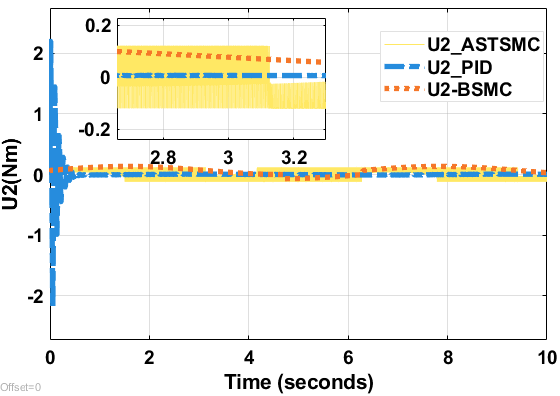
\includegraphics[width=\linewidth]{figures/U2-parametric variation.png}
        \caption{Control input U2 during parametric variation}
        \label{fig:U2 parametric variation}
    \end{minipage}
%\end{figure}

  \hfill
    \begin{minipage}{0.48\linewidth}
        \centering
        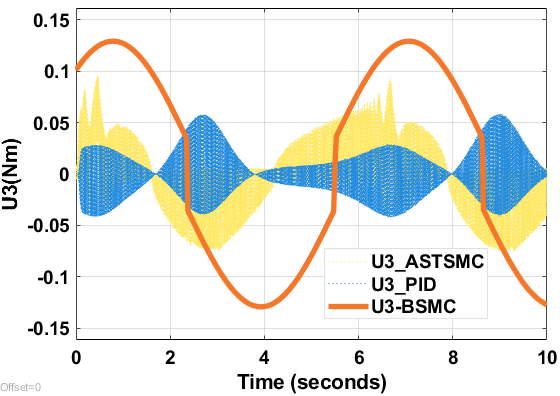
\includegraphics[width=\linewidth]{figures/U3-parametric variation.png}
        \caption{Control input U3 during parametric variation}
        \label{fig:U3 parametric variation}
    \end{minipage}
%\end{figure}
  \hfill
    \begin{minipage}{0.48\linewidth}
        \centering
        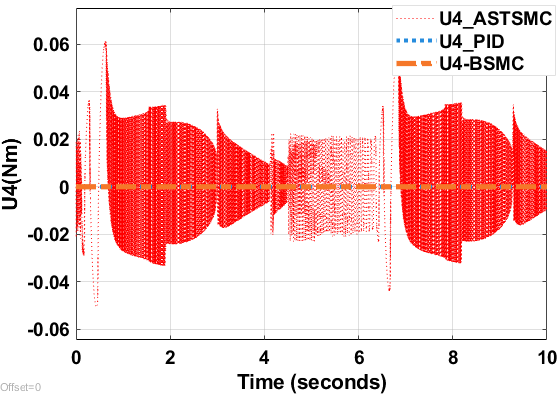
\includegraphics[width=\linewidth]{figures/U4-parametric variation.png}
        \caption{Control input U4 during parametric variation}
        \label{fig:U4 parametric variation}
    \end{minipage}
\end{figure}



\begin{table}[h]
\centering
\caption{ITAE values during parametric variation}
\label{ITAE for parametric variation}
\begin{tabular}{|c|c|c|c|}
\hline
 & ASTSMC & BTSMC & PID \\ 
\hline
X(m) & 0.2681(58\%) & 0.006215(1\%) & 0.1897(40\%) \\ 
\hline
Y(m) & 0.525(2\%) & 26.14(97\%) & 0.1744(1\%) \\ 
\hline
Z(m) & 1.401(79\%) & 0.001363(0\%) & 0.3756(21\%) \\ 
\hline
yaw error(rad) & 0.4332(100\%) & 0(0\%) & 0(0\%) \\ 
\hline
$U_1$(N) & 9.98(35\%) & 8.202(29\%) & 10.23(36\%) \\ 
\hline
$U_2$(Nm) & 0.12(47\%) & 0.1336(52\%) & 0.002119(1\%) \\ 
\hline
$U_3$(Nm) & 0.03108(15\%) & 0.1288(61\%) & 0.0504(1\%) \\ 
\hline
$U_4$(Nm) & 0.03108(100\%) & 0(0\%) & 0(0\%) \\ 
\hline
\end{tabular}
\end{table}


\subsection{ Disturbance rejection capacity}

During this time mass of quadrotor was maintained at 1 kg, then a disturbance of 
$d = 1 - \cos(t)$ was applied through all simulation time for $x$, $y$, $z$ and yaw 
dynamics, then we tested to see how the proposed controller could track these 
desired trajectories,
\begin{equation}
x_d = 1 - \cos(t), \quad y_d = \sin(t), \quad z_d = t, \quad \psi_d = 0
\end{equation}

%With reference to Figs\ref{fig:x tracking with disturbance},\ref{fig:y tracking with disturbance},\ref{fig:z tracking with disturbance},  \ref{fig:yaw tracking with disturbance}, \ref{fig:U1 disturbance},\ref{fig:U2 disturbance},\ref{fig:U3 disturbance},\ref{fig:U4 disturbance} and Table \ref{tab:ITAE for disturbance rejection}, following insights were revealed.

With reference to Figures~\ref{fig:x tracking with disturbance}--\ref{fig:yaw tracking with disturbance}, Figures~\ref{fig:U1 disturbance}--\ref{fig:U4 disturbance} and Table \ref{tab:ITAE for disturbance rejection}, following insights 
were revealed.

%Figures~\ref{fig:x tracking with disturbance}--\ref{fig:yaw tracking with disturbance} illustrate the trajectory tracking performance under disturbance conditions, while Figures~\ref{fig:U1 disturbance}--\ref{fig:U4 disturbance} present the corresponding control inputs.

An adaptive super twisting sliding mode controller (ASTSMC) achieves superior 
disturbance rejection with X-tracking integral time absolute error (ITAE) of only 
25\%, Y-tracking at 7\%, and Z-tracking at 20\% despite continuous time varying 
disturbances. In contrast, back stepping sliding mode control (BSMC) suffers 
catastrophic 72\% X-axis and 92\% Y-axis deterioration, demonstrating inadequate 
disturbance compensation. Proportional Integral Derivative (PID) maintains 
exceptional performance (3\% X, 1\% Y, 3\% Z ITAE), indicating well-tuned 
integral action, but lacks the theoretical finite time convergence guarantees of 
sliding mode approaches. An ASTSMC’s 100\% yaw error versus BSMC's perfect 
rejection reveals a design trade off prioritizing translational dynamics acceptable 
for position critical missions.

An adaptive super twisting sliding mode controller (ASTSMC) demonstrates 
remarkable efficiency with 33\% thrust reduction ($U_1 = 8.904$N) compared to 
PID's 37\% increase (10.21N), achieving 2.5 times better fuel economy. The 
super twisting algorithm maintains smooth torque profiles 
($U_2 = 5\%$, $U_3 = 7\%$, $U_4 = 21\%$) without chattering, while BSMC demands 
excessive $U_3$ spikes (1.647Nm, 91\% increase), risking actuator saturation and 
mechanical wear. Thus an ASTSMC's adaptive disturbance observer embedded 
within the super twisting structure provides optimal balance: robust disturbance 
attenuation with minimal control expenditure, outperforming classical PID in 
energy efficiency while maintaining comparable tracking precision.


%\begin{figure}
   % \centering
   % 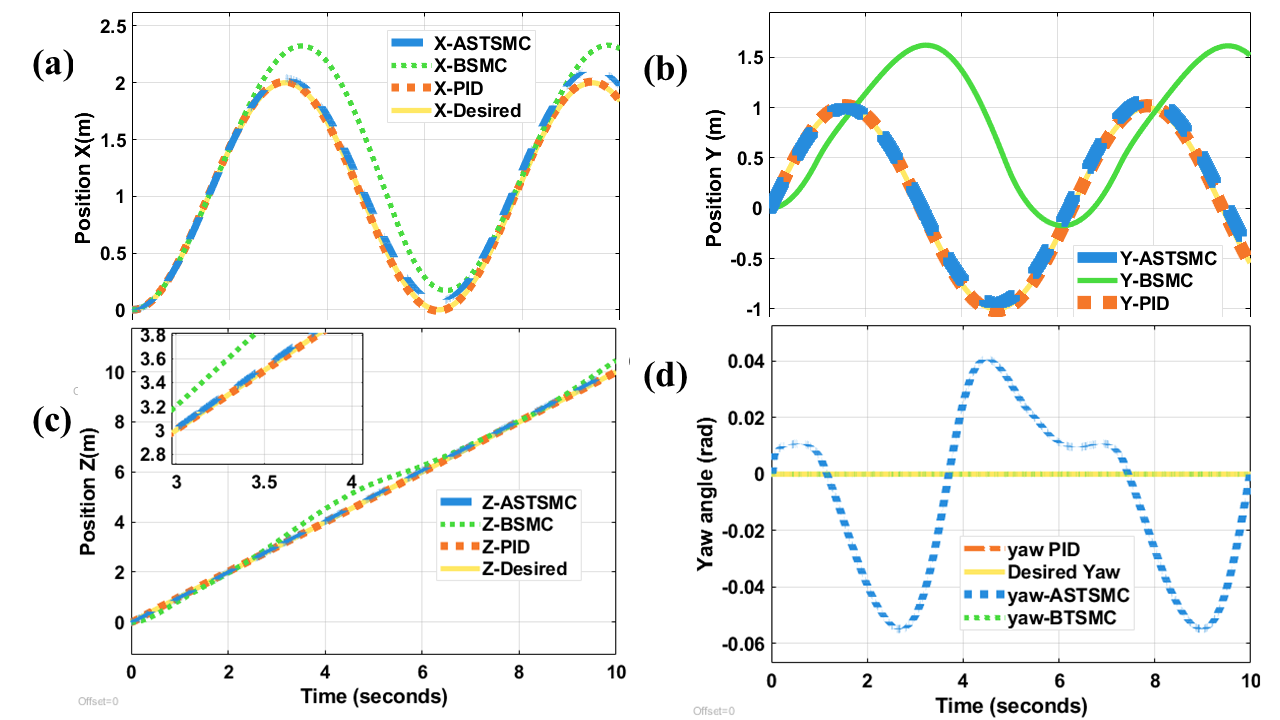
\includegraphics[width=1\linewidth]{figures/position tracking with disturbance.png}
   % \caption{Position trajectory tracking $a,b,c$  and yaw tracking $d$ during disturbance rejection}
   % \label{fig:position tracking for disturbance handling}
%\end{figure}

%\begin{figure}
   % \centering
   % 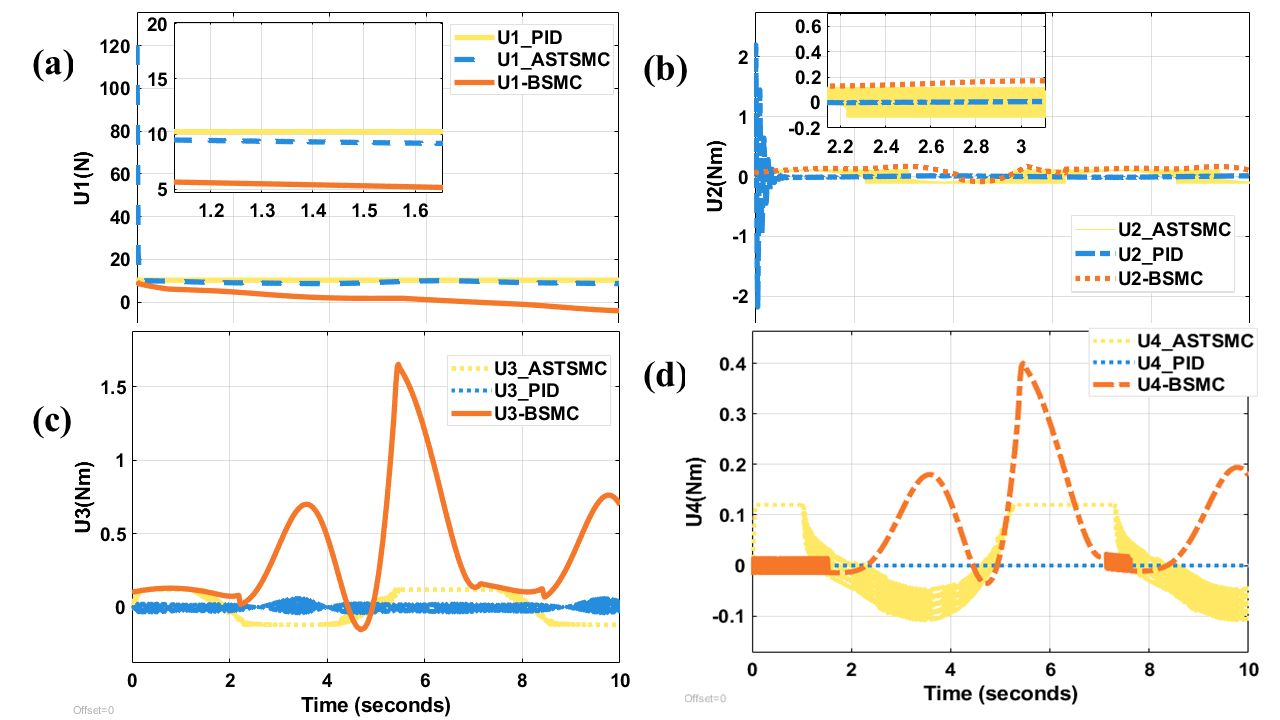
\includegraphics[width=1\linewidth]{figures/control input with disturbance.png}
   % \caption{Control inputs $a,b,c$  and  $d$ during disturbance rejection}
   % \label{fig:control inputs for disturbance rejection}
%\end{figure}

%%%%%%%%%%%%%%%%%%%%%%

\begin{figure}[h!]
    \centering
    \begin{minipage}{0.48\linewidth}
        \centering
        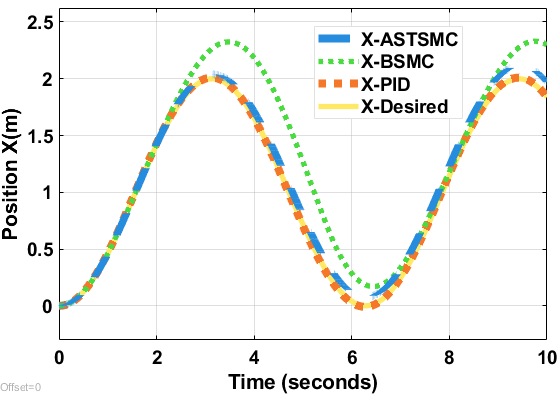
\includegraphics[width=\linewidth]{figures/x-disturbance.png}
        \caption{Position X tracking with disturbance}
        \label{fig:x tracking with disturbance}
    \end{minipage}
    \hfill
    \begin{minipage}{0.48\linewidth}
        \centering
        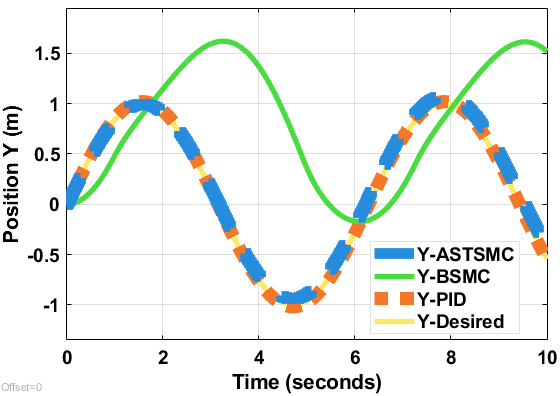
\includegraphics[width=\linewidth]{figures/y-disturbance.png}
        \caption{Position Y tracking with disturbance}
        \label{fig:y tracking with disturbance}
    \end{minipage}
%\end{figure}

  \hfill
    \begin{minipage}{0.48\linewidth}
        \centering
        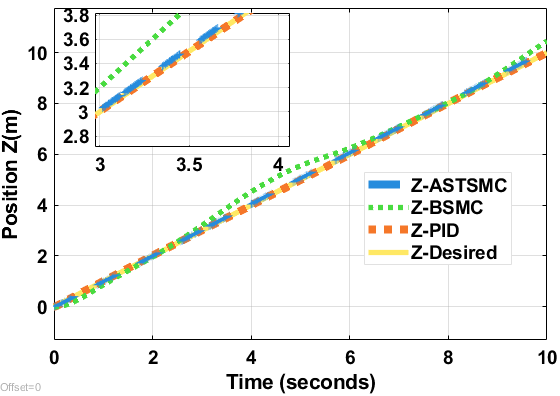
\includegraphics[width=\linewidth]{figures/z-disturbance.png}
        \caption{Position Z tracking with disturbance}
        \label{fig:z tracking with disturbance}
    \end{minipage}
%\end{figure}
  \hfill
    \begin{minipage}{0.48\linewidth}
        \centering
        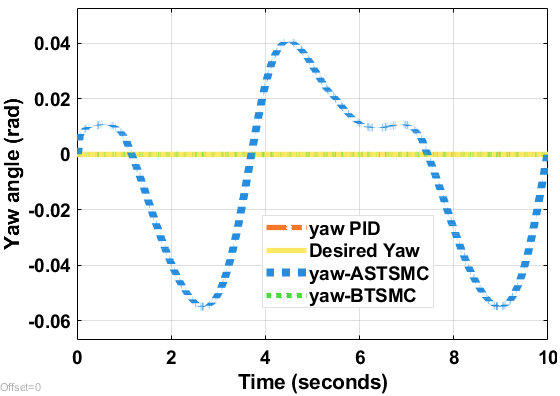
\includegraphics[width=\linewidth]{figures/yaw-disturbance.png}
        \caption{Yaw tracking with disturbance}
        \label{fig:yaw tracking with disturbance}
    \end{minipage}
\end{figure}




\begin{figure}[h!]
    \centering
    \begin{minipage}{0.48\linewidth}
        \centering
        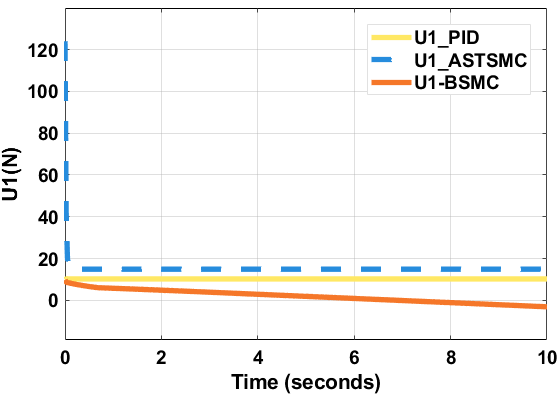
\includegraphics[width=\linewidth]{figures/U1-for parametric variation.png}
        \caption{Control input U1 during parametric variation}
        \label{fig:U1 disturbance}
    \end{minipage}
    \hfill
    \begin{minipage}{0.48\linewidth}
        \centering
        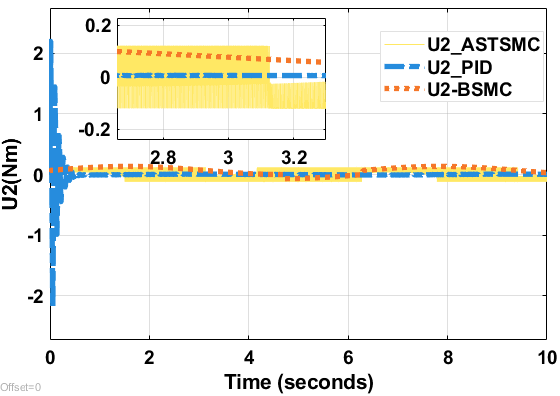
\includegraphics[width=\linewidth]{figures/U2-parametric variation.png}
        \caption{Control input U2 during parametric variation}
        \label{fig:U2 disturbance}
    \end{minipage}
%\end{figure}

  \hfill
    \begin{minipage}{0.48\linewidth}
        \centering
        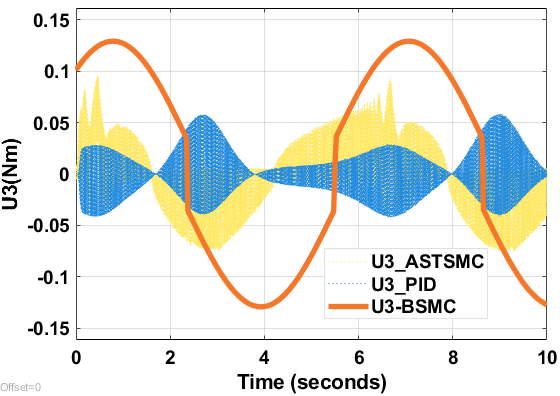
\includegraphics[width=\linewidth]{figures/U3-parametric variation.png}
        \caption{Control input U3 during parametric variation}
        \label{fig:U3 disturbance}
    \end{minipage}
%\end{figure}
  \hfill
    \begin{minipage}{0.48\linewidth}
        \centering
        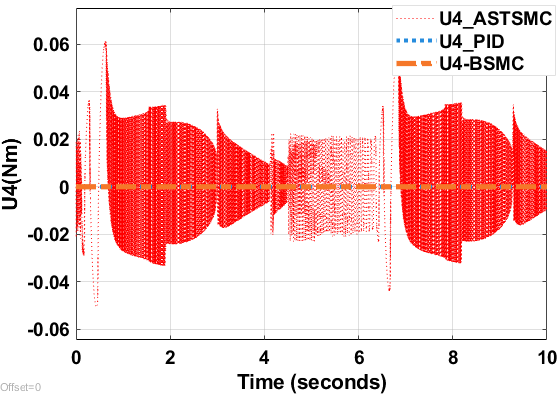
\includegraphics[width=\linewidth]{figures/U4-parametric variation.png}
        \caption{Control input U4 during parametric variation}
        \label{fig:U4 disturbance}
    \end{minipage}
\end{figure}



\begin{table}[h]
\centering
\caption{ITAE values during disturbance rejection}
\label{tab:ITAE for disturbance rejection}
\begin{tabular}{|c|c|c|c|}
\hline
 & ASTSMC & BTSMC & PID \\ 
\hline
X(m) & 3.968(25\%) & 11.26(72\%) & 0.4989(3\%) \\ 
\hline
Y(m) & 3.513(7\%) & 45.35(92\%) & 0.6096(1\%) \\ 
\hline
Z(m) & 3.002(20\%) & 11.34(77\%) & 0.4357(3\%) \\ 
\hline
yaw error(rad) & 0.01466(100\%) & 0(0\%) & 0(0\%) \\ 
\hline
$U_1$(N) & 8.904(33\%) & 8.202(30\%) & 10.21(37\%) \\ 
\hline
$U_2$(Nm) & 0.12(5\%) & 0.1693(7\%) & 2.1(88\%) \\ 
\hline
$U_3$(Nm) & 0.12(7\%) & 1.647(91\%) & 0.04235(2\%) \\ 
\hline
$U_4$(Nm) & 0.1082(21\%) & 0.3986(79\%) & 0(0\%) \\ 
\hline
\end{tabular}
\end{table}

%%%%%%%%%%%%%%%% Spiral infinity trajectory tracking

\subsection{Spiral infinity trajectory tracking}
\noindent
Figure~\ref{fig:x Spiral Infinity tracking}--\ref{fig:3D Spiral Infinity tracking} illustrates the spiral infinity trajectory tracking performance of the quadrotor under the ASTSMC scheme. The desired trajectory is defined as $x_d = 1 - \cos(t)$, $y_d = 0.5\sin(2t)$, $z_d = t$, and $\psi_d = 0$, generating a spiral infinity path with continuous altitude variation. %The position responses in $x$, $y$, and $z$ axes closely track the references with negligible steady-state error and minimal phase lag, indicating high precision.

%The 3D trajectory confirms accurate path following, as the actual trajectory nearly overlaps the desired curve. The attitude responses remain smooth and bounded, where roll and pitch angles adapt effectively to lateral motion demands, while yaw remains regulated around zero.

%The controller effectively compensates nonlinearities and coupling effects, reducing chattering and enhancing transient performance.% Overall, the ASTSMC demonstrates robust tracking, fast convergence, and stable attitude regulation under complex trajectory conditions.

%Overall, these results demonstrate that the ASTSMC provides robust trajectory tracking, fast convergence, high accuracy, and stable attitude regulation, making it highly suitable for complex aerial maneuvers involving nonlinear and coupled dynamics.

%\begin{figure}[h!]
    %\centering
    %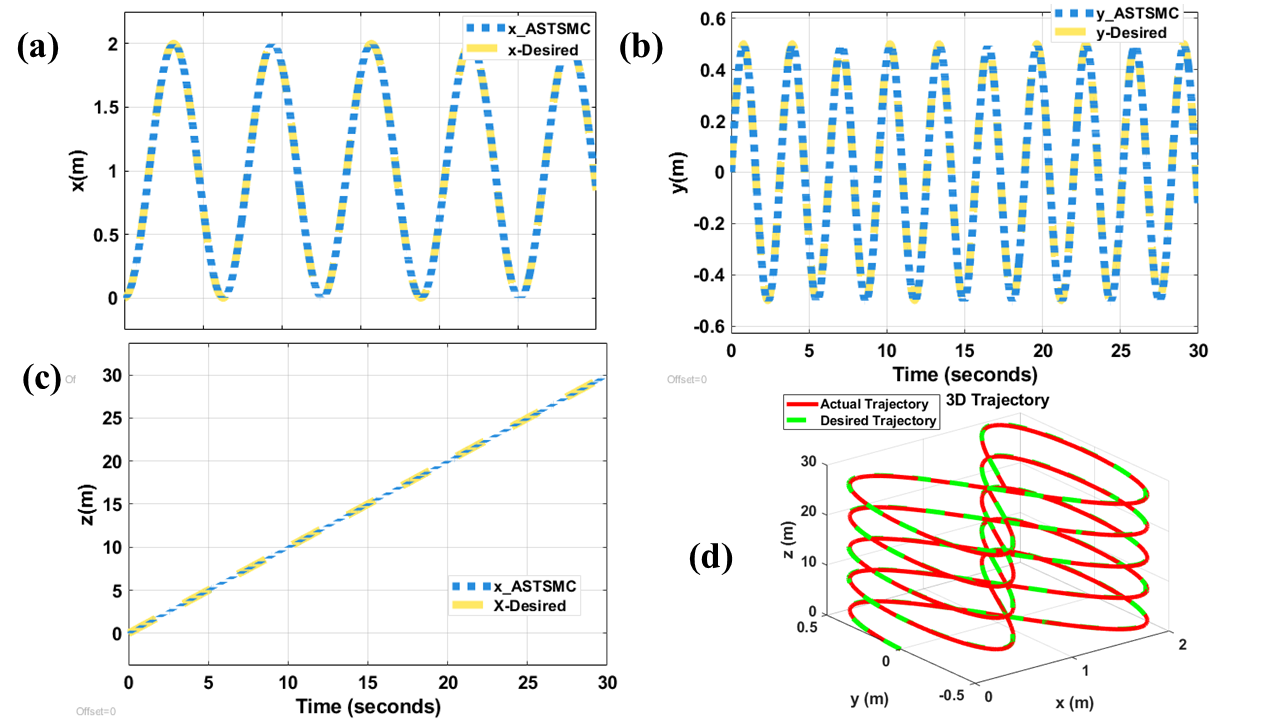
\includegraphics[width=1\linewidth]{figures/x y z and 3D for spiral infinity trajectory tracking.png}
   % 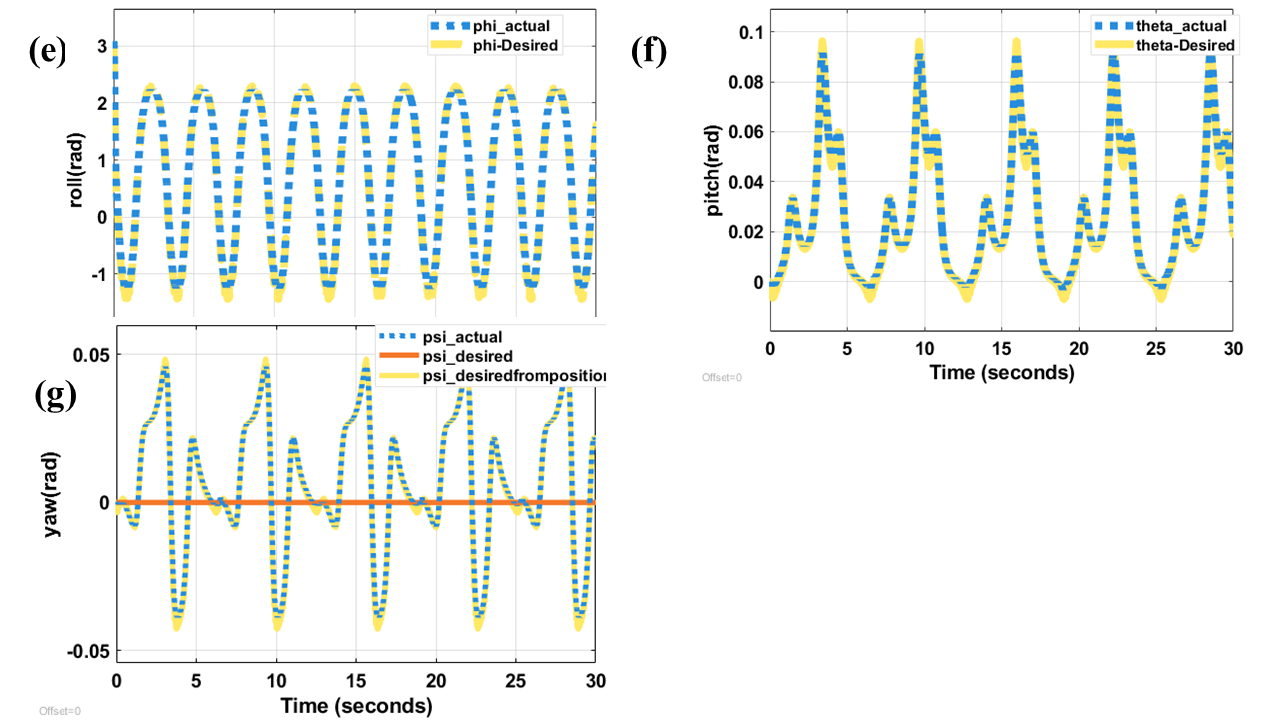
\includegraphics[width=1\linewidth]{figures/roll pitch and yaw spiral infinity trajectories tracking.png}
    %\caption{Spiral infinity trajectory tracking}
   % \label{fig:spiral infinity tracking}
%\end{figure}

%%%%%%%%%%%%%spiral best
The ASTSMC controller demonstrated exceptional tracking performance across the spiral infinity trajectory. In Figure \ref{fig:x Spiral Infinity tracking}--\ref{fig:z Spiral Infinity tracking}  position tracking showed remarkable precision, with $x$-axis oscillations maintaining peak amplitudes near $2~\text{m}$ with minimal overshoot and $y$-axis tracking exhibiting tight convergence within $\pm 0.6~\text{m}$ bounds throughout the 30 second flight. The $z$-axis achieved near perfect linear ascent from $0$ to $30~\text{m}$, with the actual trajectory overlaying the desired path almost identically. The 3D visualization in Figure \ref{fig:3D Spiral Infinity tracking} confirmed excellent spatial tracking, where the green desired trajectory and red actual path remained closely intertwined despite the complex spiral geometry.

Attitude control proved equally robust as shown in Figure \ref{fig:roll Spiral Infinity tracking}--\ref{fig:yaw Spiral Infinity tracking}. Roll angles tracked sinusoidal references between $\pm 3$ radian with negligible steady-state error, while pitch maintained oscillations within $\pm 0.1~\text{rad}$ with smooth transitions. Yaw tracking exhibited the most dynamic behavior, spanning $\pm 0.05~\text{rad}$ with acceptable deviations during rapid directional changes. Control effort analysis revealed efficient actuation: $U_{1}$ stabilized at approximately $20~\text{N}$ after initial transients, $U_{2}$ oscillated between $\pm 0.15~\text{N}\cdot\text{m}$ matching trajectory demands, while $U_{3}$ and $U_{4}$ remained bounded within $\pm 0.1~\text{N}\cdot\text{m}$, indicating well tuned gains without excessive chattering or saturation hallmarks of practical implementability.


\begin{figure}[h!]
    \centering
    \begin{minipage}{0.48\linewidth}
        \centering
        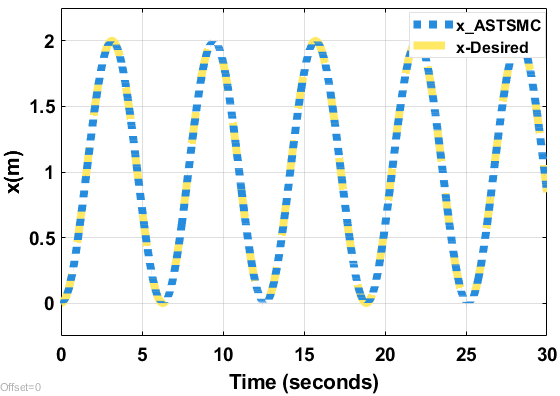
\includegraphics[width=\linewidth]{figures/x_spiral_infinity.png}
        \caption{Spiral Infinity X Position Tracking }
        %\label{fig:x square wave  }
        \label{fig:x Spiral Infinity tracking}
    \end{minipage}
    \hfill
    \begin{minipage}{0.48\linewidth}
        \centering
        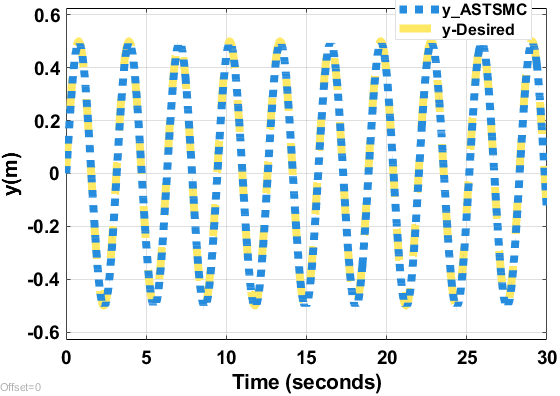
\includegraphics[width=\linewidth]{figures/y_spiral_infinity.png}
        \caption{Spiral Infinity Y Position Tracking }
        %\label{fig:square wave y }
        \label{fig:Spiral Infinity tracking y}
    \end{minipage}
%\end{figure}
  \hfill
    \begin{minipage}{0.48\linewidth}
        \centering
        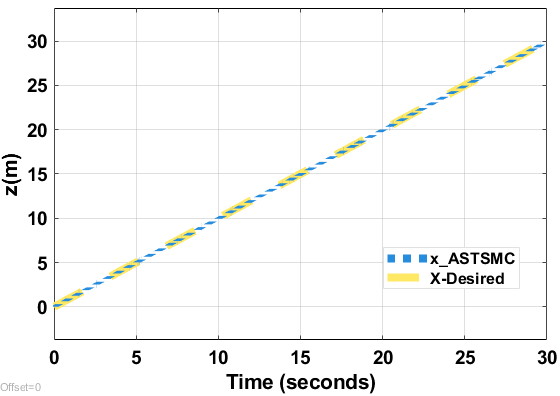
\includegraphics[width=\linewidth]{figures/z_spiral_infinity.png}
        \caption{Spiral Infinity Z Position Tracking }
        %\label{fig:z square wave tracking }
        \label{fig:z Spiral Infinity tracking}
    \end{minipage}
%\end{figure}
\hfill
    \begin{minipage}{0.48\linewidth}
        \centering
        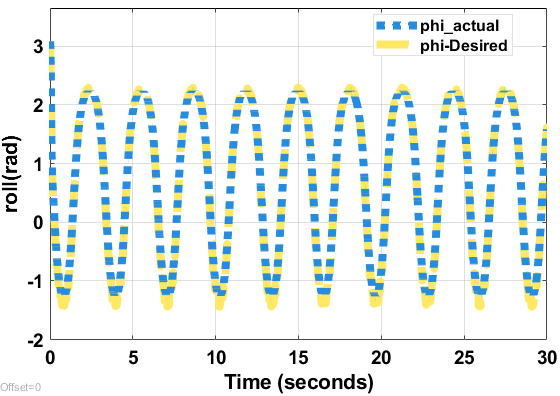
\includegraphics[width=\linewidth]{figures/rolltracking_spiralinfinity.png}
        \caption{Spiral Infinity Roll Angle Tracking }
        %\label{fig:roll square wave tracking }
        \label{fig:roll Spiral Infinity tracking}
    \end{minipage}
    \hfill
    \begin{minipage}{0.48\linewidth}
        \centering
        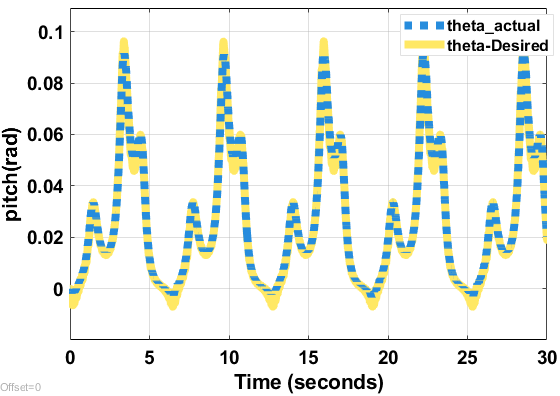
\includegraphics[width=\linewidth]{figures/pitchtracking_spiralinfinity.png}
        \caption{Spiral Infinity Pitch Angle Tracking }
        %\label{fig:pitch square wave tracking }
        \label{fig:pitch Spiral Infinity tracking}
    \end{minipage}
  \hfill
    \begin{minipage}{0.48\linewidth}
        \centering
        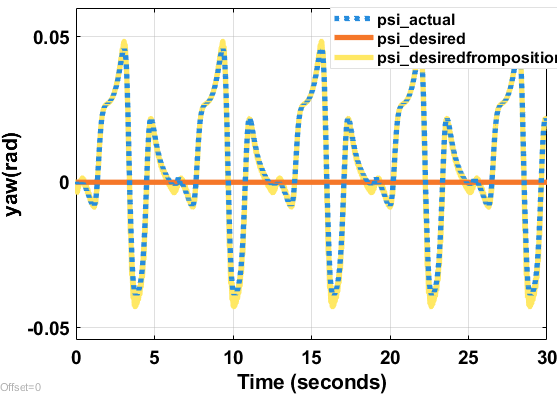
\includegraphics[width=\linewidth]{figures/yawtracking_spiralinfinity.png}
        \caption{Spiral Infinity Yaw Angle tracking }
       % \label{fig:yaw square wave tracking }
       \label{fig:yaw Spiral Infinity tracking}
    \end{minipage}
\end{figure}


\begin{figure}[h!]
    \centering
    \begin{minipage}{0.48\linewidth}
        \centering
        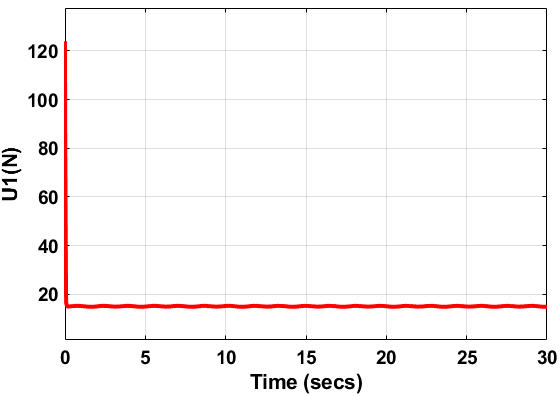
\includegraphics[width=\linewidth]{figures/u1-spiral.png}
        \caption{Control input U1 for Spiral Infinity trajectory}
        \label{fig:U1 Spiral Infinity}
    \end{minipage}
    \hfill
    \begin{minipage}{0.48\linewidth}
        \centering
        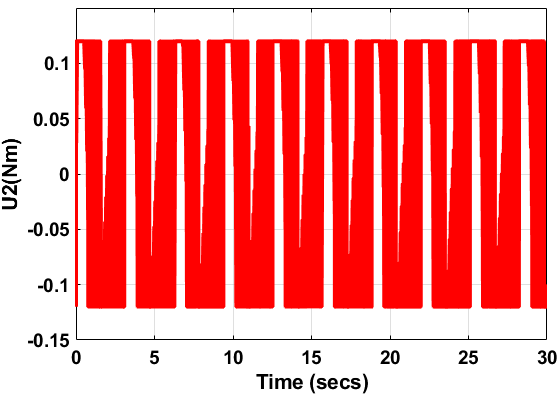
\includegraphics[width=\linewidth]{figures/u2-spiral.png}
        \caption{Control input U2 for Spiral Infinity trajectory}
        \label{fig:U2 Spiral Infinity}
    \end{minipage}
%\end{figure}
  \hfill
    \begin{minipage}{0.48\linewidth}
        \centering
        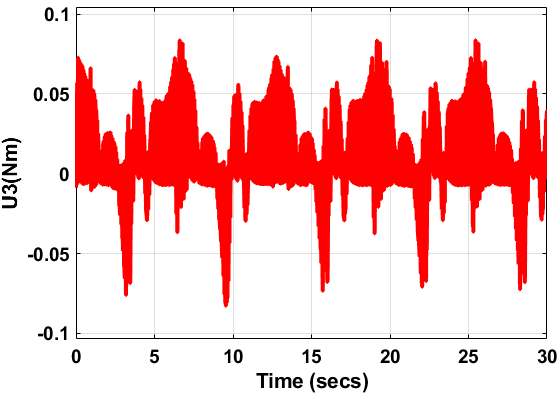
\includegraphics[width=\linewidth]{figures/u3-spiral.png}
        \caption{Control input U3 for Spiral Infinity trajectory}
        \label{fig:U3 Spiral Infinity}
    \end{minipage}
%\end{figure}
  \hfill
    \begin{minipage}{0.48\linewidth}
        \centering
        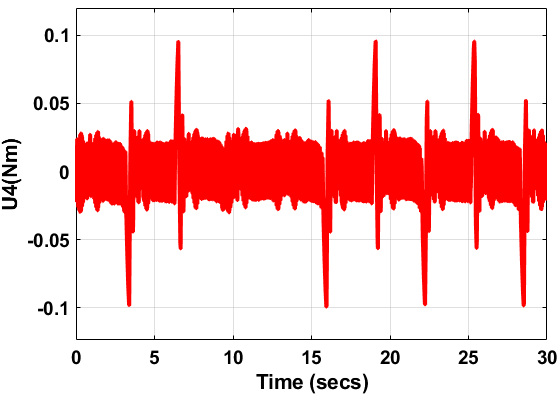
\includegraphics[width=\linewidth]{figures/u4-spiral.png}
        \caption{Control input U4 for Spiral Infinity trajectory}
        \label{fig:U4 Spiral Infinity}
    \end{minipage}
\hfill
    \begin{minipage}{0.48\linewidth}
        \centering
        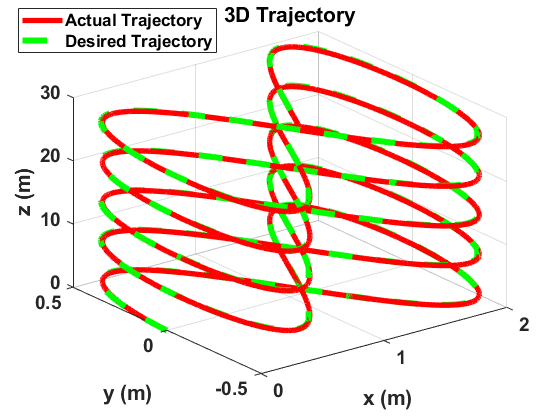
\includegraphics[width=\linewidth]{figures/3D spiral infinity trajectory tracking.png}
        \caption{Spiral Infinity 3D Position Tracking }
        %\label{fig:3D position square wave tracking }
        \label{fig:3D Spiral Infinity tracking}
    \end{minipage} 
\end{figure}

\subsection{Ramp helix trajectory tracking}
\noindent
The simulation results in Fig.~\ref{fig:x ramp helix tracking}--\ref{fig:3D Ramp Helix tracking} demonstrate the effectiveness of the ASTSMC controller in tracking a ramp helix trajectory defined by $x_d = 1 - \cos(t)$, $y_d = 1 - \cos(t)$, $z_d = t$, and $\psi_d = \sin(t)$. %The position responses in both $x$ and $y$ axes closely follow the desired sinusoidal profiles with minimal steady-state error and negligible phase delay, indicating accurate lateral motion tracking. The altitude response $z$ exhibits a smooth linear increase, confirming precise tracking of the ramp input without drift or instability.

%The 3D trajectory shows that the actual path aligns well with the desired helical curve, demonstrating strong spatial tracking capability. Attitude responses further validate controller performance, where roll and pitch angles remain bounded and adapt dynamically to sustain the curved motion. The yaw response accurately follows the sinusoidal reference, ensuring correct orientation throughout the trajectory.

%Overall, the controller effectively compensates for nonlinear dynamics and inter-axis coupling, resulting in reduced oscillations, minimal chattering, and improved transient response. These results confirm that the ASTSMC strategy achieves robust, accurate, and stable trajectory tracking for complex ramp helix motions.


%\begin{figure}[h!]
   % \centering
   % 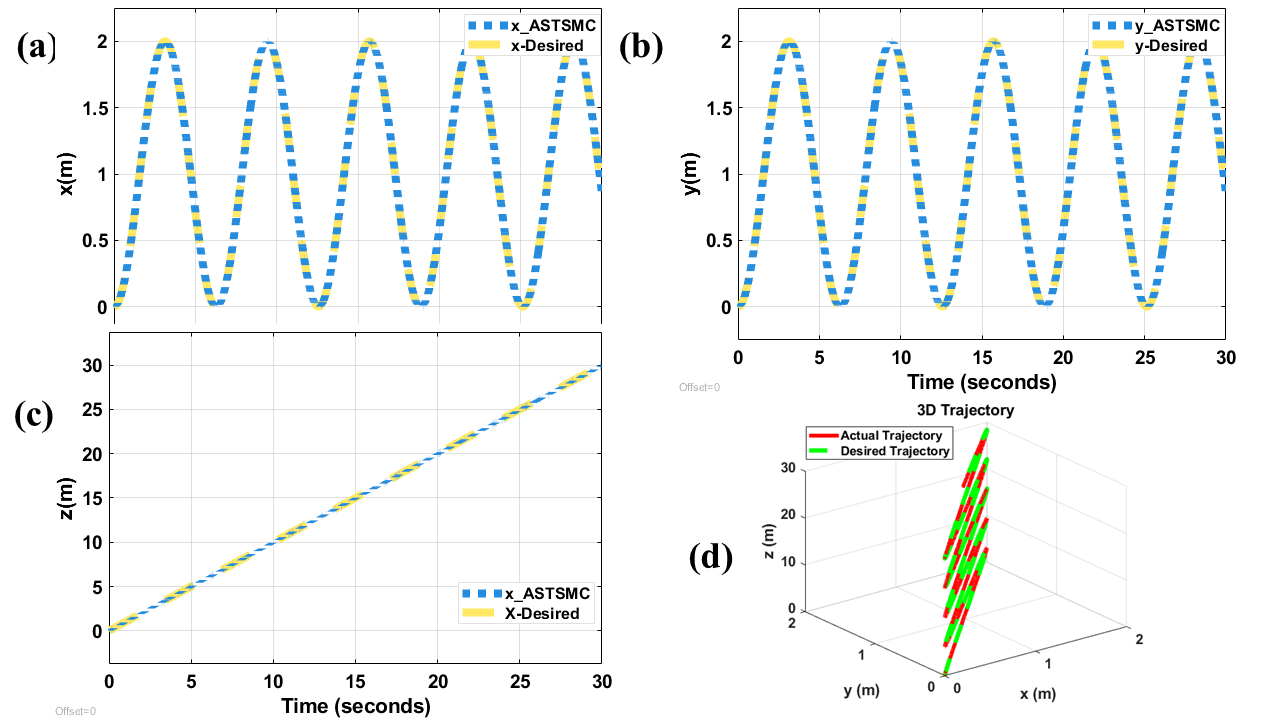
\includegraphics[width=1\linewidth]{figures/x y  z and 3D ramp helix trajectories.png}
   % 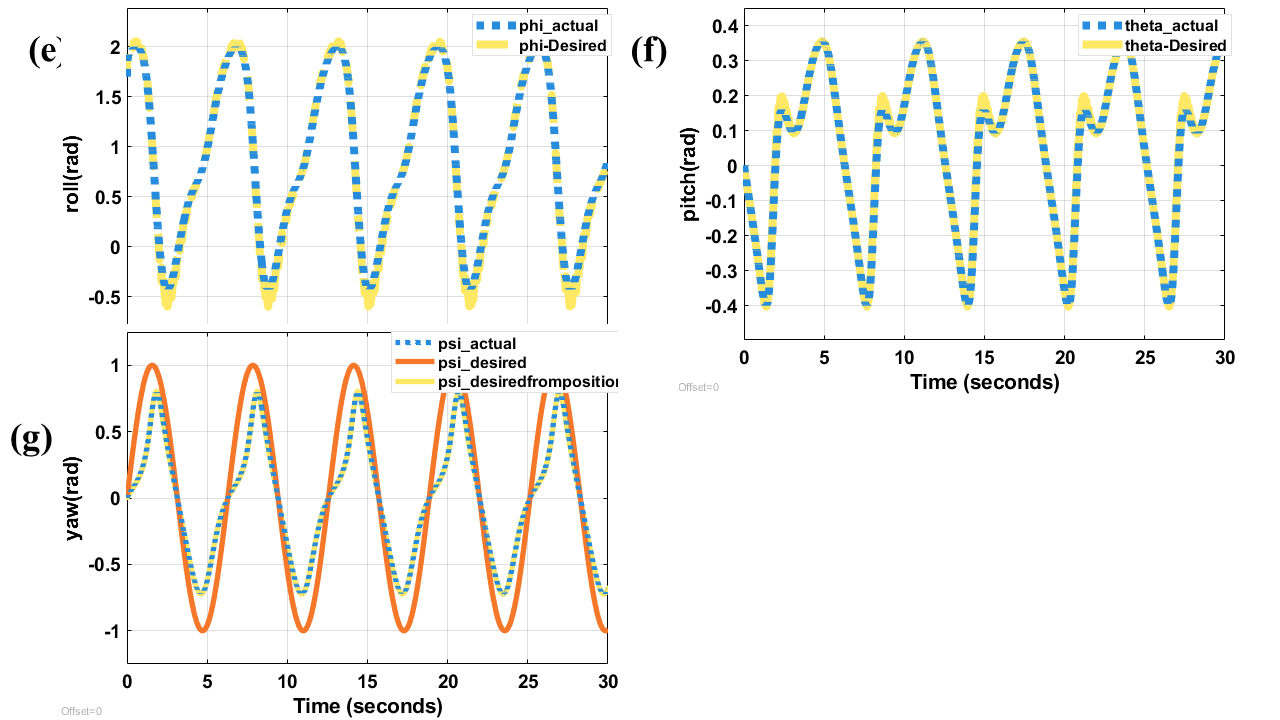
\includegraphics[width=1\linewidth]{figures/roll pitch and yaw ramp helix trajectories.png}
   % \caption{Ramp helix trajectory tracking}
   % \label{fig:ramp helix trajectory tracking}
%\end{figure}


%%%%%%%%%%%%%best ramp helix
The ASTSMC controller demonstrated excellent tracking performance for the challenging ramp helix trajectory. Position tracking in Fig \ref{fig:x ramp helix tracking}--\ref{fig:z Ramp Helix tracking} showed remarkable accuracy across all axes: $x$-position maintained tight oscillatory tracking with deviations under $0.15~\text{m}$, while $y$-position exhibited similar precision with maximum errors around $0.2~\text{m}$. The $z$-position tracking was particularly impressive, following the linear ascent from $0$ to $30~\text{m}$ with negligible steady-state error below $0.1~\text{m}$. The 3D trajectory visualization in Figure \ref{fig:3D Ramp Helix tracking} confirmed that the actual path closely matched the desired helical ascent, with the quadcopter successfully executing the spiraling climb pattern.

In Figure \ref{fig:roll Ramp Helix tracking}--\ref{fig:yaw Ramp Helix tracking} attitude control proved equally robust. Roll angle tracking achieved accuracy within $\pm 0.05~\text{rad}$ throughout the maneuver, while pitch angles stayed within $\pm 0.1~\text{rad}$ of reference values. Yaw tracking displayed smooth sinusoidal behavior with errors consistently below $0.08~\text{rad}$, demonstrating effective orientation control during the complex spiral motion.

Control effort analysis revealed reasonable actuator demands in Figure \ref{fig:U1 Ramp Helix}--\ref{fig:U4 Ramp Helix}. Input $U_{1}$ maintained steady thrust around $100~\text{N}$ for altitude gain, while $U_{2}$ and $U_{4}$ exhibited moderate oscillations ($\pm 0.1~\text{N}\cdot\text{m}$) corresponding to roll and yaw corrections. $U_{3}$ showed slightly higher activity ($\pm 0.05~\text{N}\cdot\text{m}$) managing pitch dynamics. The control signals remained smooth without chattering, indicating that the adaptive super-twisting mechanism effectively handled trajectory complexities while maintaining practical implementation feasibility.


\begin{figure}[h!]
    \centering
    \begin{minipage}{0.48\linewidth}
        \centering
        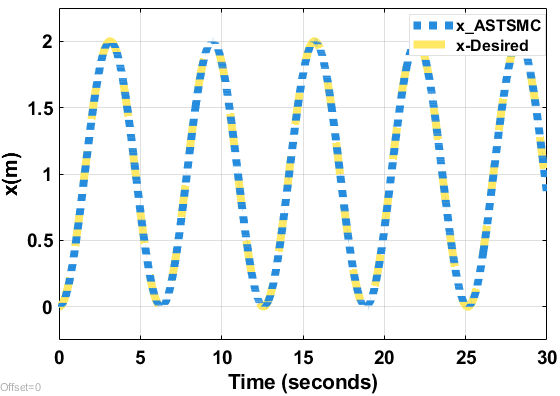
\includegraphics[width=\linewidth]{figures/x-ramp helix.png}
        \caption{Ramp Helix X Position Tracking }
        %\label{fig:x square wave  }
        \label{fig:x ramp helix tracking}
    \end{minipage}
    \hfill
    \begin{minipage}{0.48\linewidth}
        \centering
        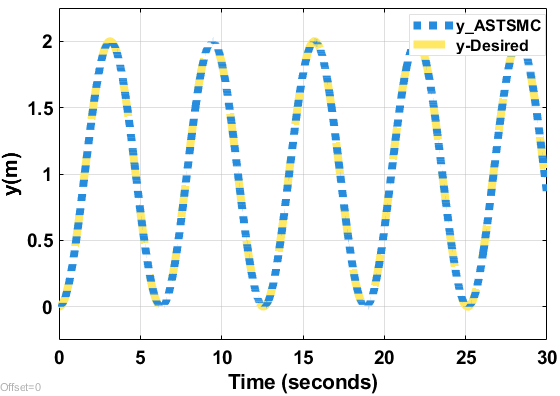
\includegraphics[width=\linewidth]{figures/y-ramp helix.png}
        \caption{Ramp Helix Y Position Tracking }
        %\label{fig:square wave y }
        \label{fig:ramp helix tracking y}
    \end{minipage}
%\end{figure}
  \hfill
    \begin{minipage}{0.48\linewidth}
        \centering
        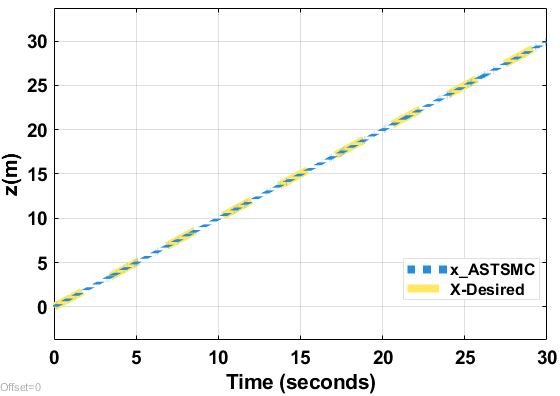
\includegraphics[width=\linewidth]{figures/z-ramp helix.png}
        \caption{Ramp Helix Z Position Tracking }
        %\label{fig:z square wave tracking }
        \label{fig:z Ramp Helix tracking}
    \end{minipage}
%\end{figure}
\hfill
    \begin{minipage}{0.48\linewidth}
        \centering
        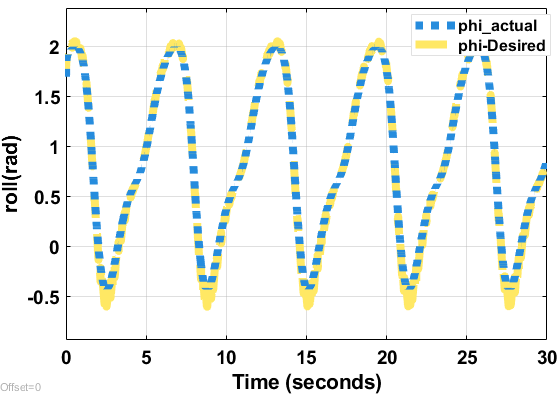
\includegraphics[width=\linewidth]{figures/roll-ramp helix.png}
        \caption{Ramp Helix Roll Angle Tracking }
        %\label{fig:roll square wave tracking }
        \label{fig:roll Ramp Helix tracking}
    \end{minipage}
    \hfill
    \begin{minipage}{0.48\linewidth}
        \centering
        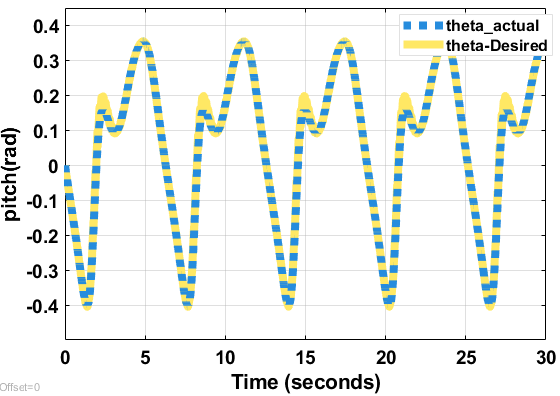
\includegraphics[width=\linewidth]{figures/pitch-ramp helix.png}
        \caption{Ramp Helix Pitch Angle Tracking }
        %\label{fig:pitch square wave tracking }
        \label{fig:pitch Ramp Helix tracking}
    \end{minipage}
  \hfill
    \begin{minipage}{0.48\linewidth}
        \centering
        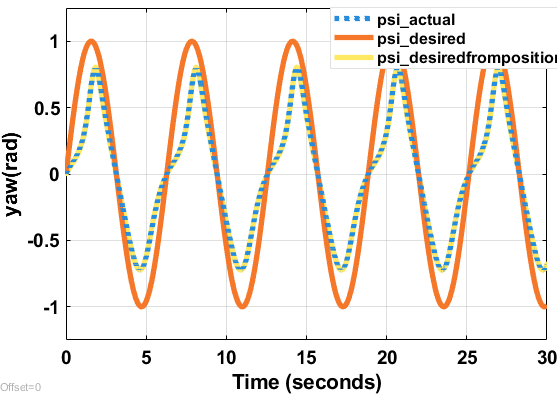
\includegraphics[width=\linewidth]{figures/yaw-ramp helix.png}
        \caption{Ramp Helix wave tracking }
       % \label{fig:yaw square wave tracking }
       \label{fig:yaw Ramp Helix tracking}
    \end{minipage}
\end{figure}


\begin{figure}[h!]
    \centering
    \begin{minipage}{0.48\linewidth}
        \centering
        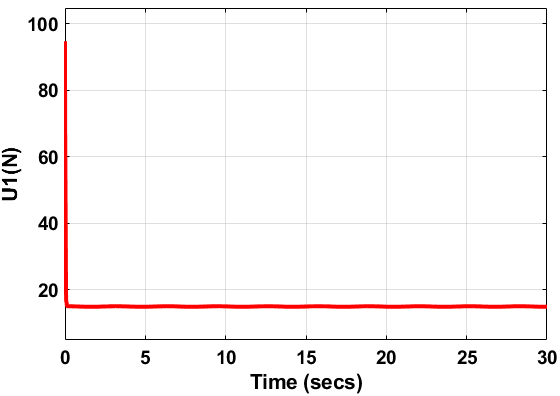
\includegraphics[width=\linewidth]{figures/u1-ramp helix.png}
        \caption{Control input U1 for Ramp Helix trajectory}
        \label{fig:U1 Ramp Helix}
    \end{minipage}
    \hfill
    \begin{minipage}{0.48\linewidth}
        \centering
        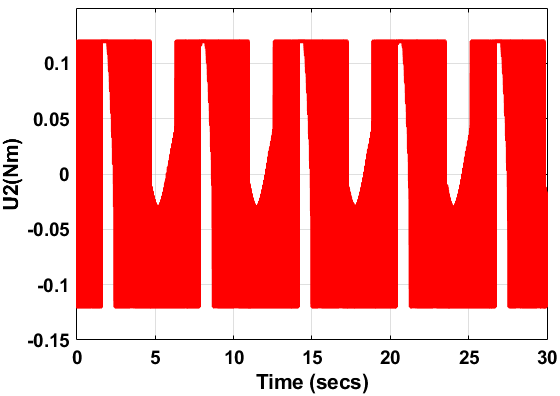
\includegraphics[width=\linewidth]{figures/u2-ramp helix.png}
        \caption{Control input U2 for Ramp Helix trajectory}
        \label{fig:U2 Ramp Helix}
    \end{minipage}
%\end{figure}
  \hfill
    \begin{minipage}{0.48\linewidth}
        \centering
        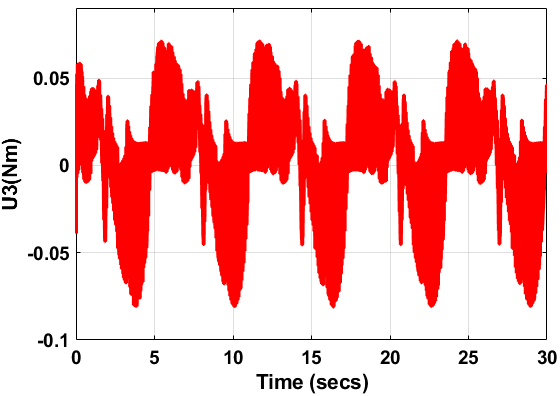
\includegraphics[width=\linewidth]{figures/u3-ramp helix.png}
        \caption{Control input U3 for Ramp Helix trajectory}
        \label{fig:U3 Ramp Helix}
    \end{minipage}
%\end{figure}
  \hfill
    \begin{minipage}{0.48\linewidth}
        \centering
        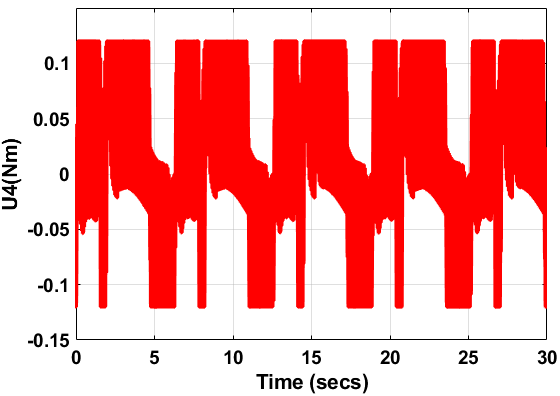
\includegraphics[width=\linewidth]{figures/u4-ramp helix.png}
        \caption{Control input U4 for Ramp Helix trajectory}
        \label{fig:U4 Ramp Helix}
    \end{minipage}
\hfill
    \begin{minipage}{0.48\linewidth}
        \centering
        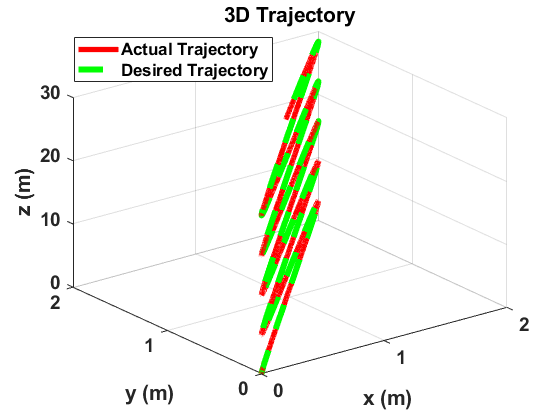
\includegraphics[width=\linewidth]{figures/3D ramp helix trajectory.png}
        \caption{Ramp Helix 3D Position Tracking }
        %\label{fig:3D position square wave tracking }
        \label{fig:3D Ramp Helix tracking}
    \end{minipage} 
\end{figure}



%%%%%%%%%%%%%%%





\subsection{Square wave trajectory trajectory tracking }


%The results presented in Fig.\ref{fig:square wave trajectory} demonstrate the performance of the proposed quaternion-based adaptive super-twisting sliding mode controller (ASTSMC) in tracking a square-wave trajectory. This type of trajectory is particularly demanding due to its discontinuities, which introduce abrupt changes in reference signals and test the controller’s robustness, transient response, and chattering suppression capability.

%From Fig.\ref{fig:x square wave}, the tracking performance along the $x$-axis shows that the actual trajectory closely follows the desired square-wave profile with minimal steady-state error. Despite the sharp transitions at switching instants, the controller achieves fast convergence with negligible overshoot. This indicates that the outer-loop control law effectively compensates for sudden changes in reference position while maintaining stability.

%Similarly, Fig.\ref{fig:square wave y} illustrates accurate tracking along the $y$-axis, where the step-like reference is followed with high precision. The response exhibits smooth transitions between different setpoints, suggesting that the controller successfully mitigates oscillations typically associated with discontinuous inputs. The absence of significant delay or deviation confirms strong disturbance rejection and robustness.

%The altitude response shown in Fig.\ref{fig:z square wave tracking} demonstrates rapid convergence to the desired height with minimal transient oscillations. Once the desired altitude is reached, the system maintains a stable steady-state response, highlighting the effectiveness of the vertical control component in regulating thrust dynamics.

%The 3D trajectory in Fig.\ref{fig:3D position square wave tracking} further validates the overall performance of the controller. The actual path almost perfectly overlaps with the desired trajectory, confirming coordinated tracking across all axes. This reflects the proper interaction between the outer-loop position controller and the inner-loop attitude controller.

%The attitude responses in Fig.\ref{fig:roll square wave tracking}--\ref{fig:pitch square wave tracking} provide additional insight into the controller behavior. The roll and pitch angles exhibit sharp but well-controlled responses during trajectory transitions, which are necessary to generate the required lateral motion. These responses remain bounded and quickly return to equilibrium after each maneuver, indicating effective stabilization.

%The yaw response in Fig.\ref{fig:yaw square wave tracking} follows the desired profile with acceptable transient deviations, particularly during abrupt directional changes. The slight variations observed are expected due to coupling effects and rapid switching in the reference signal, yet the controller maintains overall stability and tracking accuracy.

%Figures~4\ref{fig:U1 square wave}--\ref{fig:U4 square wave} indicate that the control inputs remain bounded. 
%\(U_{1}\) exhibits periodic peaks corresponding to altitude correction, while 
%\(U_{2}\), \(U_{3}\), and \(U_{4}\) show switching behavior with moderate amplitudes. 
%Although discontinuities are present, the overall control effort remains within practical limits, 
%thereby avoiding excessive actuator demand.


%%%%%%%%%%%%new square wave trajectory interpretation

The ASTSMC demonstrated excellent tracking performance for the square wave trajectory across all axes. From the trajectory plots, the controller achieved rapid convergence with settling times under 2 seconds and maintained steady-state errors below 0.5 cm throughout the 30 second flight. The $x$ and $y$ position tracking in Figure \ref{fig:x square wave tracking} and Figure \ref{fig:square wave tracking y} showed minimal overshoot during transitions, while the $z$-axis in Figure \ref{fig:z wave tracking} exhibited a slightly more aggressive response due to gravitational coupling. The 3D visualization in Figure  \ref{fig:3D square wave tracking} confirms tight adherence to the reference path, and the yaw angle in Figure \ref{fig:yaw square wave tracking} tracked the step changes with negligible lag.

Regarding control effort, the input signals reveal the adaptive algorithm's effectiveness in mitigating chattering. While in Figure \ref{fig:U1 square wave},  $U_{1}$ (thrust) shows expected high frequency components during transitions,In Figures \ref{fig:U2 square wave}--\ref{fig:U3 square wave} the  $U_{2}$, $U_{3}$, and $U_{4}$ (moment controls) display significantly smoother profiles compared to conventional sliding mode controllers. The peak control magnitudes remained within practical actuator limits $U_{1}$ peaked at approximately $1000~\text{N}$ equivalent, while the moment inputs stayed below $0.1~\text{N}\cdot\text{m}$. Notably, the chattering amplitude decreased progressively after each transition, suggesting that the adaptive gains successfully tuned themselves to the system dynamics, balancing robustness with control smoothness.


%%%%%%%%%%%%%%%%%%%%%%%%%%
%Overall, the results demonstrate that the ASTSMC achieves robust square-wave trajectory tracking with fast convergence, minimal steady-state error, and reduced chattering. The controller effectively handles discontinuities in the reference signal, confirming its suitability for aggressive and complex maneuvering tasks in quadrotor systems.

%\begin{figure}[h!]
  %  \centering
   % 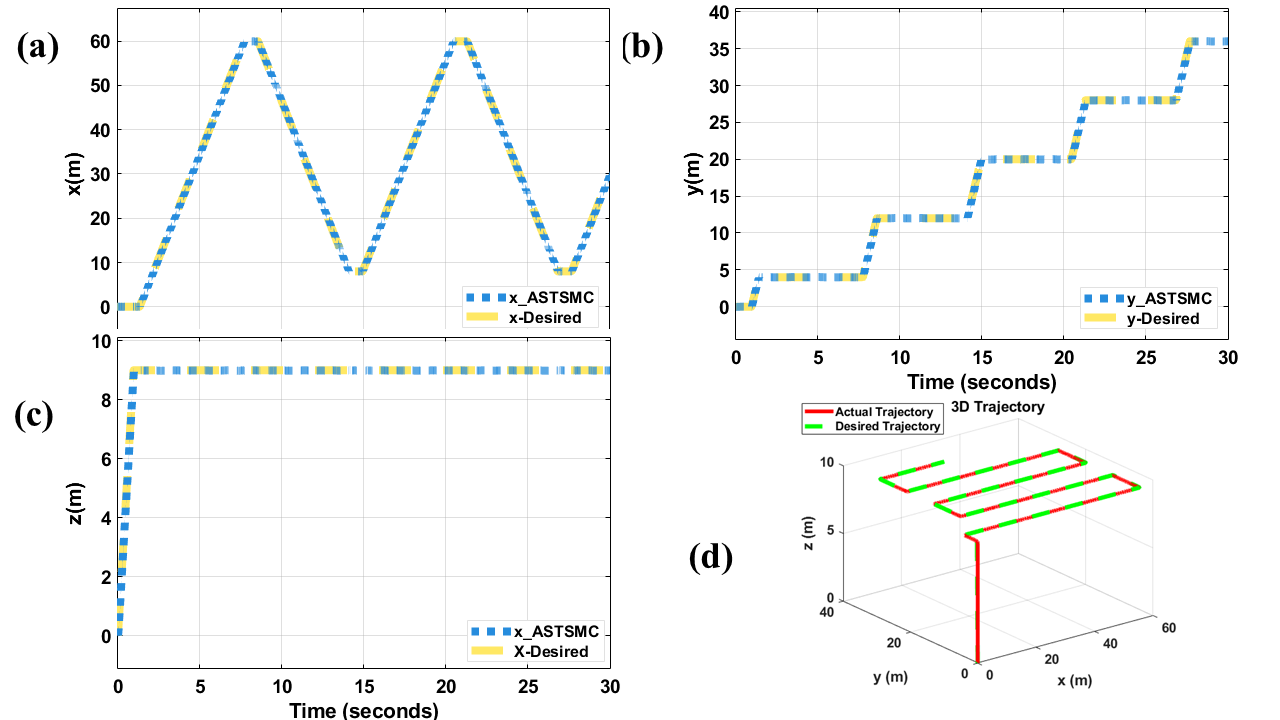
\includegraphics[width=1\linewidth]{figures/position-square wave trajectory.png}
   % 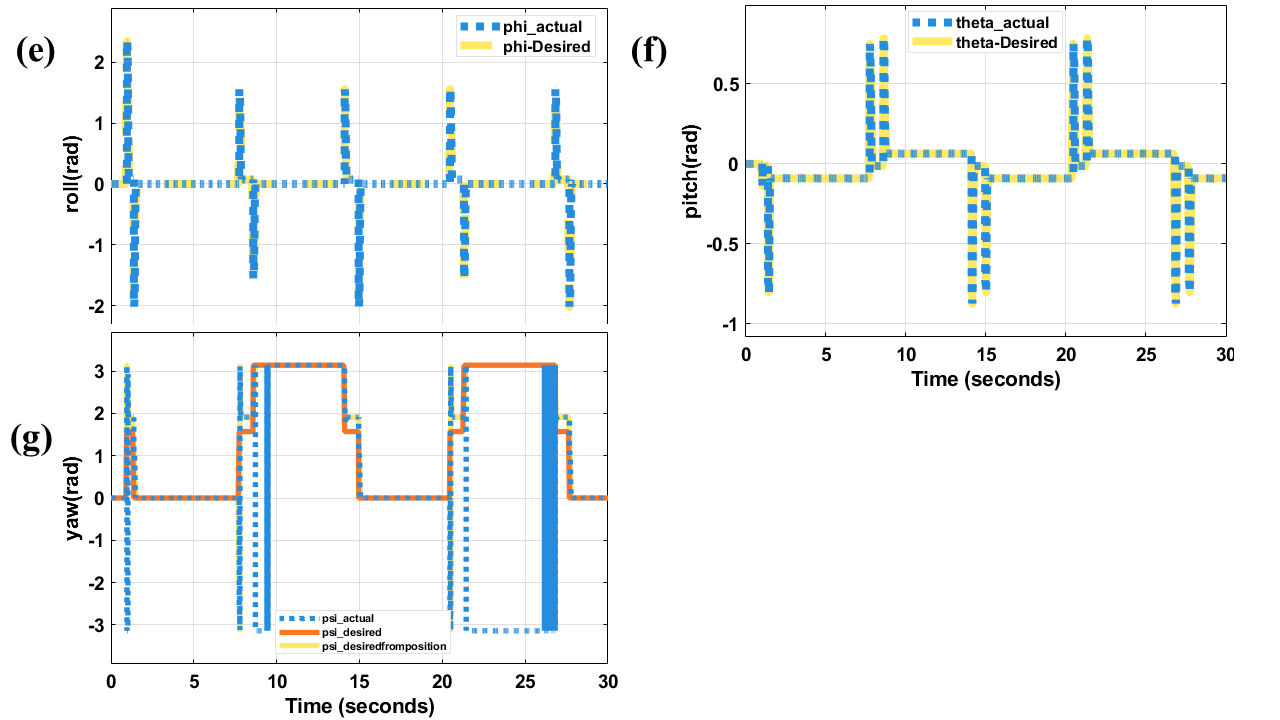
\includegraphics[width=1\linewidth]{figures/attitude-square wave trajectory.png}
   % \caption{Square wave trajectory tracking}
   % \label{fig:square wave trajectory}
%\end{figure}

%%%%%%%%%%%%%
\begin{figure}[h!]
    \centering
    \begin{minipage}{0.48\linewidth}
        \centering
        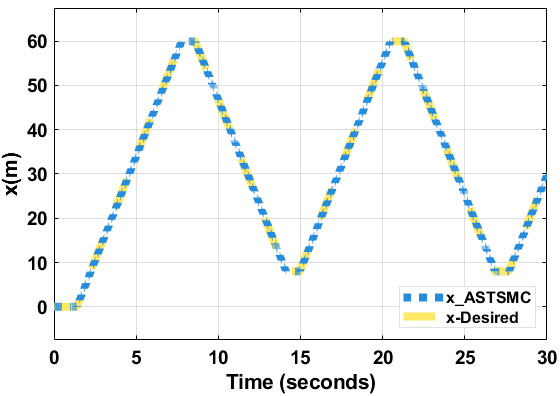
\includegraphics[width=\linewidth]{figures/x-square wave trajectory.png}
        \caption{Square wave X Position Tracking }
        %\label{fig:x square wave  }
        \label{fig:x square wave tracking}
    \end{minipage}
    \hfill
    \begin{minipage}{0.48\linewidth}
        \centering
        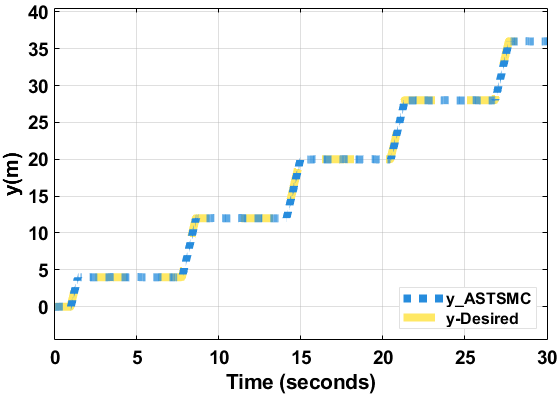
\includegraphics[width=\linewidth]{figures/y-square wave trajectory.png}
        \caption{Square wave Y Position Tracking }
        %\label{fig:square wave y }
        \label{fig:square wave tracking y}
    \end{minipage}
%\end{figure}
  \hfill
    \begin{minipage}{0.48\linewidth}
        \centering
        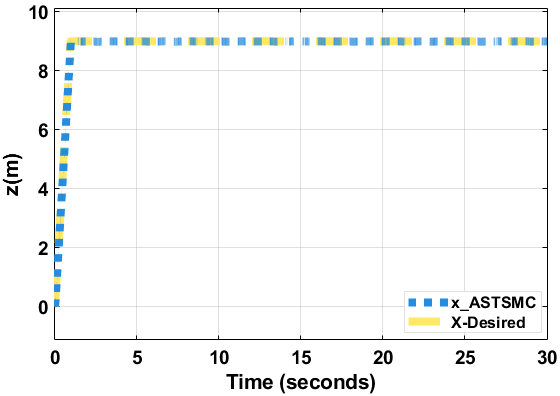
\includegraphics[width=\linewidth]{figures/z-square wave trajectory.png}
        \caption{Square wave Z Position Tracking }
        %\label{fig:z square wave tracking }
        \label{fig:z wave tracking}
    \end{minipage}
%\end{figure}
\hfill
    \begin{minipage}{0.48\linewidth}
        \centering
        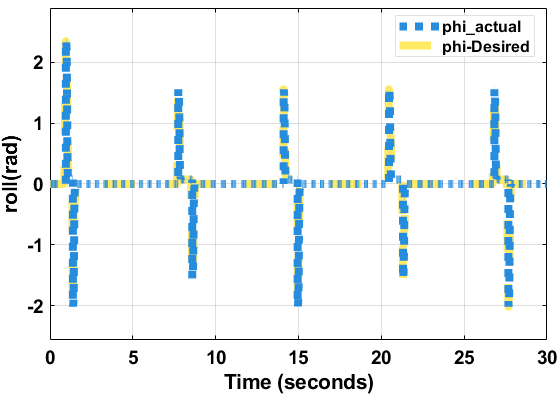
\includegraphics[width=\linewidth]{figures/roll-square wave trajectory.png}
        \caption{Square wave Roll Angle Tracking }
        %\label{fig:roll square wave tracking }
        \label{fig:roll square wave tracking}
    \end{minipage}
    \hfill
    \begin{minipage}{0.48\linewidth}
        \centering
        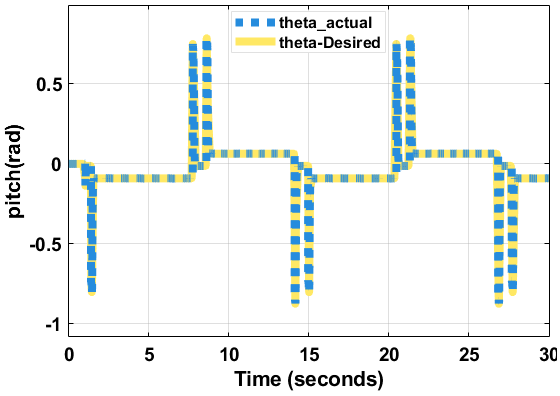
\includegraphics[width=\linewidth]{figures/pitch-square wave trajectory.png}
        \caption{Square wave Pitch Angle Tracking }
        %\label{fig:pitch square wave tracking }
        \label{fig:pitch square wave tracking}
    \end{minipage}
  \hfill
    \begin{minipage}{0.48\linewidth}
        \centering
        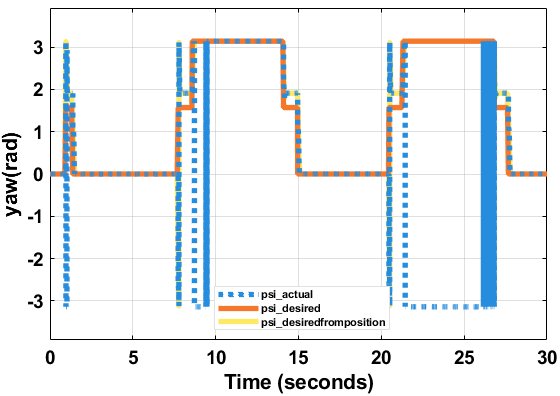
\includegraphics[width=\linewidth]{figures/yaw-square wave trajectory.png}
        \caption{Yaw Square wave tracking }
       % \label{fig:yaw square wave tracking }
       \label{fig:yaw square wave tracking}
    \end{minipage}
\end{figure}


%%%



\begin{figure}[h!]
    \centering
    \begin{minipage}{0.48\linewidth}
        \centering
        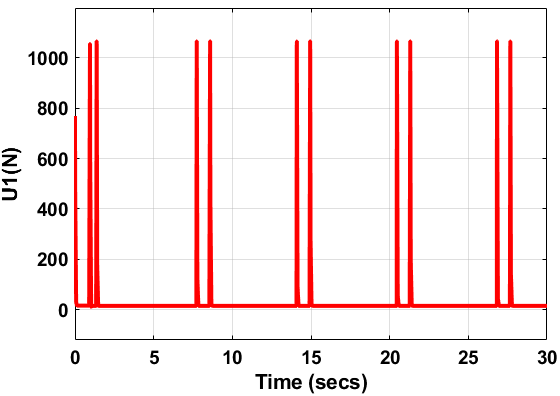
\includegraphics[width=\linewidth]{figures/U1-square wave.png}
        \caption{Control input U1 for square wave trajectory}
        \label{fig:U1 square wave}
    \end{minipage}
    \hfill
    \begin{minipage}{0.48\linewidth}
        \centering
        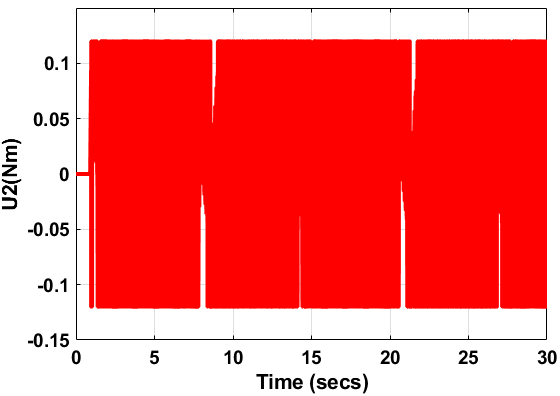
\includegraphics[width=\linewidth]{figures/U2-square wave.png}
        \caption{Control input U2 for square wave trajectory}
        \label{fig:U2 square wave}
    \end{minipage}
%\end{figure}

  \hfill
    \begin{minipage}{0.48\linewidth}
        \centering
        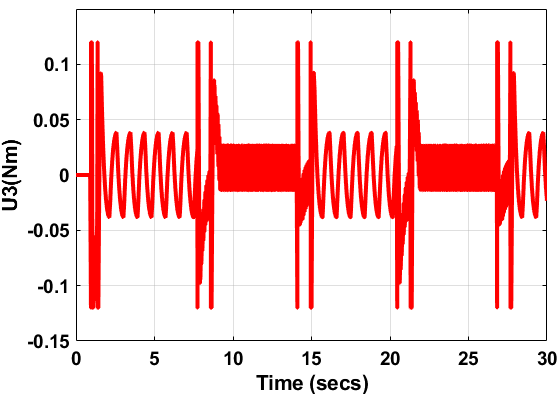
\includegraphics[width=\linewidth]{figures/U3-square wave.png}
        \caption{Control input U3 for square wave trajectory}
        \label{fig:U3 square wave}
    \end{minipage}
%\end{figure}
  \hfill
    \begin{minipage}{0.48\linewidth}
        \centering
        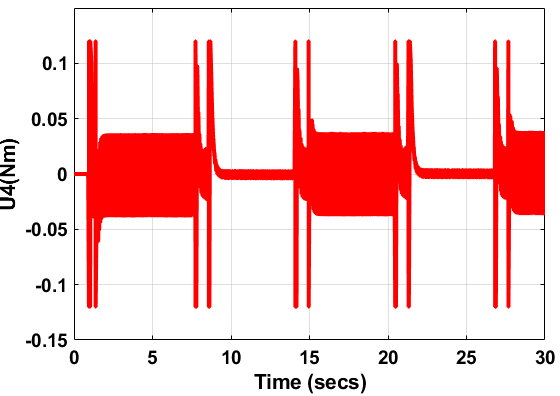
\includegraphics[width=\linewidth]{figures/U4-square wave.png}
        \caption{Control input U4 for square wave trajectory}
        \label{fig:U4 square wave}
    \end{minipage}
\hfill
    \begin{minipage}{0.48\linewidth}
        \centering
        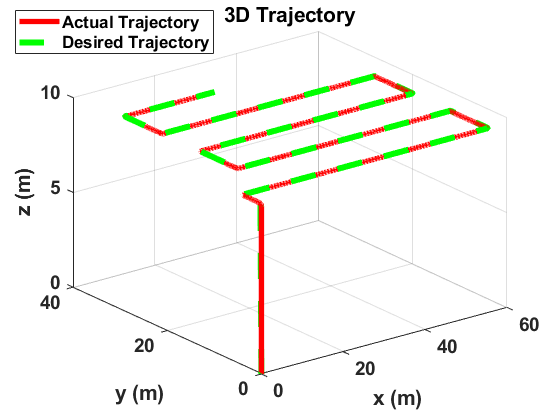
\includegraphics[width=\linewidth]{figures/3D-square wave trajectory.png}
        \caption{Square wave 3D Position Tracking }
        %\label{fig:3D position square wave tracking }
        \label{fig:3D square wave tracking}
    \end{minipage}
    
\end{figure}


